% ******************************* PhD Thesis Template **************************
% Please have a look at the README.md file for info on how to use the template

\documentclass[a4paper,12pt,numbered,print,index,custommargin, PageStyleII,  twoside]{Classes/PhDThesisPSnPDF}

% ******************************************************************************
% ******************************* Class Options ********************************
% *********************** See README for more details **************************
% ******************************************************************************

% `a4paper'(The University of Cambridge PhD thesis guidelines recommends a page
% size a4 - default option) or `a5paper': A5 Paper size is also allowed as per
% the Cambridge University Engineering Deparment guidelines for PhD thesis
%
% `11pt' or `12pt'(default): Font Size 10pt is NOT recommended by the University
% guidelines
%
% `oneside' or `twoside'(default): Printing double side (twoside) or single
% side.
%
% `print': Use `print' for print version with appropriate margins and page
% layout. Leaving the options field blank will activate Online version.
%
% `index': For index at the end of the thesis
%
% `draftclassic': For draft mode without loading any images (same as draft in book)
%
% `draft': Special draft mode with line numbers, images, and water mark with
% timestamp and custom text. Position of the text can also be modified.
%
% `abstract': To generate only the title page and abstract page with
% dissertation title and name, to submit to the Student Registry
%
% `chapter`: This option enables only the specified chapter and it's references
%  Useful for review and corrections.
%
% ************************* Custom Page Margins ********************************
%
% `custommargin`: Use `custommargin' in options to activate custom page margins,
% which can be defined in the preamble.tex. Custom margin will override
% print/online margin setup.
%
% *********************** Choosing the Fonts in Class Options ******************
%
% `times' : Times font with math support. (The Cambridge University guidelines
% recommend using times)
%
% `fourier': Utopia Font with Fourier Math font (Font has to be installed)
%            It's a free font.
%
% `customfont': Use `customfont' option in the document class and load the
% package in the preamble.tex
%
% default or leave empty: `Latin Modern' font will be loaded.
%
% ********************** Choosing the Bibliography style ***********************
%
% `authoryear': For author-year citation eg., Krishna (2013)
%
% `numbered': (Default Option) For numbered and sorted citation e.g., [1,5,2]
%
% `custombib': Define your own bibliography style in the `preamble.tex' file.
%              `\RequirePackage[square, sort, numbers, authoryear]{natbib}'.
%              This can be also used to load biblatex instead of natbib
%              (See Preamble)
%
% **************************** Choosing the Page Style *************************
%
% `default (leave empty)': For Page Numbers in Header (Left Even, Right Odd) and
% Chapter Name in Header (Right Even) and Section Name (Left Odd). Blank Footer.
%
% `PageStyleI': Chapter Name next & Page Number on Even Side (Left Even).
% Section Name & Page Number in Header on Odd Side (Right Odd). Footer is empty.
%
% `PageStyleII': Chapter Name on Even Side (Left Even) in Header. Section Number
% and Section Name in Header on Odd Side (Right Odd). Page numbering in footer

% ********************************** Preamble **********************************
% Preamble: Contains packages and user-defined commands and settings
% ******************************************************************************
% ****************************** Custom Margin *********************************

% Add `custommargin' in the document class options to use this section
% Set {innerside margin / outerside margin / topmargin / bottom margin}  and
% other page dimensions
\ifsetCustomMargin
  \RequirePackage[left=30mm,right=25mm,top=25mm,bottom=25mm]{geometry}
  \setFancyHdr % To apply fancy header after geometry package is loaded
\fi

% Add spaces between paragraphs
%\setlength{\parskip}{1em} - see after \begin{document}

% Ragged bottom avoids extra whitespaces between paragraphs
\raggedbottom
% To remove the excess top spacing for enumeration, list and description
%\usepackage{enumitem}
%\setlist[enumerate,itemize,description]{topsep=0em}

% *****************************************************************************
% ******************* Fonts (like different typewriter fonts etc.)*************

% Add `customfont' in the document class option to use this section

\ifsetCustomFont
  % Set your custom font here and use `customfont' in options. Leave empty to
  % load computer modern font (default LaTeX font).
  %\RequirePackage{helvet}

  % For use with XeLaTeX
  %  \setmainfont[
  %    Path              = ./libertine/opentype/,
  %    Extension         = .otf,
  %    UprightFont = LinLibertine_R,
  %    BoldFont = LinLibertine_RZ, % Linux Libertine O Regular Semibold
  %    ItalicFont = LinLibertine_RI,
  %    BoldItalicFont = LinLibertine_RZI, % Linux Libertine O Regular Semibold Italic
  %  ]
  %  {libertine}
  %  % load font from system font
  %  \newfontfamily\libertinesystemfont{Linux Libertine O}
\fi

% *****************************************************************************
% **************************** Custom Packages ********************************

% ************************* Algorithms and Pseudocode **************************

\usepackage{algpseudocode}


% ********************Captions and Hyperreferencing / URL **********************

% Captions: This makes captions of figures use a boldfaced small font.
\RequirePackage[small,bf]{caption}

\RequirePackage[,tableposition=top]{caption} % labelsep=space for space 
\renewcommand{\figurename}{Figure} %to support older versions of captions.sty

% *************************** Graphics and figures *****************************

%\usepackage{rotating}
%\usepackage{wrapfig}

% Uncomment the following two lines to force Latex to place the figure.
% Use [H] when including graphics. Note 'H' instead of 'h'
\usepackage{graphbox}
\usepackage{float}
\restylefloat{figure}

% Subcaption package is also available in the sty folder you can use that by
% uncommenting the following line
% This is for people stuck with older versions of texlive
%\usepackage{sty/caption/subcaption}
\usepackage{subcaption}

% ********************************** Tables ************************************
\usepackage{booktabs} % For professional looking tables
\usepackage{multirow}

\usepackage{multicol}
\usepackage{longtable}
\usepackage{tabularx}
\usepackage{parskip}

% *********************************** SI Units *********************************
\usepackage{siunitx} % use this package module for SI units


% ******************************* Line Spacing *********************************

% Choose linespacing as appropriate. Default is one-half line spacing as per the
% University guidelines

% \doublespacing
% \onehalfspacing
% \singlespacing


% ************************ Formatting / Footnote *******************************

% Don't break enumeration (etc.) across pages in an ugly manner (default 10000)
\clubpenalty=500
\widowpenalty=500

\usepackage[bottom]{footmisc} 
% `perpage`: Range of footnote options, reset to 1 per page
% `bottom`: sticks footnote to the end of page regardless



% *****************************************************************************
% *************************** Bibliography  and References ********************

%\usepackage{cleveref} %Referencing without need to explicitly state fig /table

% Add `custombib' in the document class option to use this section
\ifuseCustomBib
%   \RequirePackage[square, sort, numbers, authoryear]{natbib} % CustomBib

% If you would like to use biblatex for your reference management, as opposed to the default `natbibpackage` pass the option `custombib` in the document class. Comment out the previous line to make sure you don't load the natbib package. Uncomment the following lines and specify the location of references.bib file

\RequirePackage[backend=biber, style=numeric-comp, citestyle=numeric, sorting=nty, natbib=true]{biblatex}
\addbibresource{References/references} %Location of references.bib only for biblatex, Do not omit the .bib extension from the filename.
\fi

% changes the default name `Bibliography` -> `References'
%\renewcommand{\bibname}{References}


% ******************************************************************************
% ************************* User Defined Commands ******************************
% ******************************************************************************

% *********** To change the name of Table of Contents / LOF and LOT ************

\renewcommand{\contentsname}{Contents}
%\renewcommand{\listfigurename}{My List of Figures}
%\renewcommand{\listtablename}{My List of Tables}


% ********************** TOC depth and numbering depth *************************

% Uncomment the next 2 lines to add dots to TOC
%\usepackage{tocloft}  
%\renewcommand{\cftchapleader}{\cftdotfill{\cftdotsep}} 
\setcounter{secnumdepth}{2}
\setcounter{tocdepth}{2}


% ******************************* Nomenclature *********************************

% To change the name of the Nomenclature section, uncomment the following line

%\renewcommand{\nomname}{Symbols}


% ********************************* Appendix ***********************************

% The default value of both \appendixtocname and \appendixpagename is `Appendices'. These names can all be changed via:

%\renewcommand{\appendixtocname}{List of appendices}
%\renewcommand{\appendixname}{Appndx}
\usepackage{docmute} % only needed to allow inclusion of proposal.tex

% *********************** Configure Draft Mode **********************************

% Uncomment to disable figures in `draft'
%\setkeys{Gin}{draft=true}  % set draft to false to enable figures in `draft'

% These options are active only during the draft mode
% Default text is "Draft"
%\SetDraftText{DRAFT}

% Default Watermark location is top. Location (top/bottom)
%\SetDraftWMPosition{bottom}

% Draft Version - default is v1.0
%\SetDraftVersion{v1.1}

% Draft Text grayscale value (should be between 0-black and 1-white)
% Default value is 0.75
%\SetDraftGrayScale{0.8}


% ******************************** Todo Notes **********************************
%% Uncomment the following lines to have todonotes.

%\ifsetDraft
%	\usepackage[colorinlistoftodos]{todonotes}
%	\newcommand{\mynote}[1]{\todo[author=kks32,size=\small,inline,color=green!40]{#1}}
%\else
%	\newcommand{\mynote}[1]{}
%	\newcommand{\listoftodos}{}
%\fi

% Example todo: \mynote{Hey! I have a note}

% *****************************************************************************
% ******************* Better enumeration my MB*************
\usepackage{enumitem}

% ************************ Thesis Information & Meta-data **********************
% Thesis title and author information, refernce file for biblatex
% ************************ Thesis Information & Meta-data **********************
%% The title of the thesis
\title{An accelerated, network-assisted TCP fast retransmit}

%% Subtitle (Optional)
\subtitle{Computer Science Tripos - Part II Project}

%% The full name of the author
\author{Thanh Bui}

%% Department (eg. Department of Engineering, Maths, Physics)
\dept{Department of Computer Science}

%% University and Crest
\university{University of Cambridge}


% Crest minimum should be 30mm.
\crest{
	\noindent
	\begin{minipage}{0.3\textwidth}% adapt widths of minipages to your needs
				
\includegraphics[width=\textwidth, align=t]{University_Crest_Long.pdf}
	\end{minipage}%
	\hfill%
	\begin{minipage}{0.72\textwidth}\raggedleft
		\begin{singlespace}
			\vspace*{10mm}
			\large \textit{Thanh Bui}
			\\[0pt]
			\large \textit{Downing College}
			\\[0pt]
			\texttt{ttb29}
		\end{singlespace}
	\end{minipage}
}

%% Supervisor (optional) - commented out for dissertation
%\supervisor{Dr Noa Zilberman}

%% College affiliation (optional)
\college{Downing College}

%% Submission date
\degreedate{May 17, 2019} 

%% Meta information
\subject{LaTeX} \keywords{{LaTeX} {PhD Thesis} {Engineering} {University of
Cambridge}}


\begin{document}
\setlength{\parskip}{0.75\baselineskip}

\maketitle

% ******************************** Proforma & Declaration *********************************

\section*{Declaration}

I, Thanh Bui of Downing College, being a candidate for Part II of the Computer Science Tripos, hereby declare that this dissertation and the work described in it are my own work, unaided except as may be specified below, and that the dissertation does not contain material that has already been used to any substantial extent for a comparable purpose.

\begin{minipage}[t]{0.4\textwidth}
	\vspace*{1.5cm}  % leave some space above the horizontal line
	\hrule
	\vspace{1mm} % just a bit more whitespace below the line
	\begin{tabular}[t]{l}
		SIGNED
	\end{tabular}
\end{minipage} 
\hspace{2cm}
\begin{minipage}[t]{0.4\textwidth}
	\vspace*{1.5cm}  % leave some space above the horizontal line
	\hrule
	\vspace{1mm} % just a bit more whitespace below the line
	\begin{tabular}[t]{l}
		DATE
	\end{tabular}
\end{minipage}

\chapter*{Proforma}

{\large
\begin{tabular}{ l@{\hskip 3.25em} p{11cm}}
	Candidate Number:               & \bf Thanh Bui \\
	College:            & \bf Downing College \\
	Project Title:      & \bf An accelerated, network-assisted TCP fast retransmit \\
\end{tabular}
}
\\
{\large
\begin{tabular}{ l p{11.5cm}}
	Examination:        & \bf Computer Science Tripos --- Part II, June 2019  \\
	Word Count:         & \bf 11000\footnotemark	 \\
	Project Originator: & Dr Noa Zilberman               \\
	Supervisor:         & Dr Noa Zilberman             		\\ 
\end{tabular}
}
\footnotetext{This word count was computed using \texttt{texcount -sum -inc -utf8 -sub=chapter diss.tex} for chapters 1--5.
}

\section*{Original Aims of the Project}
The aim of this project is to investigate the feasibility and effectiveness of a programmable data plane in application to Transmission Control Protocol (TCP) congestion control. More specifically, I aim to design, implement and evaluate a programmable switch to recover from TCP packet losses that are not due to congestion. The implementation will be evaluated based on a series of tests, including both software and hardware simulations. A performance evaluation will also be provided.  

\section*{Work Completed}
Almost all my success criteria were met, with the exception of demonstrating the interoperability of my implementation with a software-based client/application. The architecture was designed, then implemented in P4. The implementation was tested via three different simulations: SDNet simulation, SUME simulation and hardware simulation. A performance evaluation of the design was provided. Two of the extensions were also completed. 

\section*{Special Difficulties}
The implementation stage of the architecture took longer than anticipated due to limitations of SDNet and the P4$\rightarrow$NetFPGA workflow. The current P4$\rightarrow$NetFPGA only supports header processing, without deep packet inspection, while this project used programmable buffering logic, which would require the ability to buffer packets. Hence, the design could not be fully expressed in P4 alone. To circumvent this, I had to learn to use Verilog in order to design a different architecture by adding additional HDL modules into the framework that allow packet buffering. 

% ******************************** TOC *********************************

\tableofcontents
\listoffigures
%\listoftables

% ******************************** Main Diss *********************************

\chapter{Introduction}
\textit{In this chapter, I provide the motivation for this project and setup the problem I am solving. I also explain some key algorithms involved. Finally, I cover some related work.}

\section{Motivation}
	
 Transmission Control Protocol (TCP) is the protocol of choice in many data centers. However, it is very sensitive to losses (by design, as a mean for congestion control), which can degrade the performance within the data centers significantly \cite{zilberman2017has}. Various congestion control, avoidance and recovery mechanisms are thus of high importance in this field to minimise such loss rate. Still, not all TCP losses are born equal. For example, losses happening at the destination host's network interface card (NIC) are not an indication of congestion within the network. It is assumed that fast retransmission of such lost packets, from within the network, can increase the utilization of the network.
 
 In-network computing is an emerging research area in systems and networking, where applications traditionally running on the host are offloaded to the network hardware (e.g. switch, NIC). Examples of applications offloaded in the past include network functions (DNS server \cite{dns}), distributed systems functions such as consensus (P4xos \cite{p4xos}), various caching (netCache \cite{netCache}, netChain \cite{netChain}) and even a game (Tic-Tac-Toe). Key-Value Store (KVS) is also among the popular type of in-network applications. 
 
 Therefore, it is particularly interesting, and indeed challenging, to see how network-accelerated KVS concepts can be applied to TCP fast retransmit mechanism in order to improve cross-datacentre performance.
 
\section{Project Aims}
Fast retransmit is an enhancement to TCP that reduces the time a sender waits before retransmitting a lost segment. A TCP sender normally uses a simple timer to recognize lost segments. If an acknowledgement is not received for a particular segment within a specified time (a function of the estimated round-trip delay time), the sender will assume the segment was lost in the network, and will retransmit the segment.

Duplicate acknowledgement (DUP ACK) is the basis for the fast retransmit mechanism. After receiving a packet (e.g. with sequence number 1), the receiver sends an acknowledgement by adding 1 to the sequence number (i.e. acknowledgement number 2). This indicates to the sender that the receiver received the packet number 1 and it expects packet number 2. Suppose that three subsequent packets are lost. The next packets the receiver sees are packet numbers 5 and 6. After receiving packet number 5, the receiver sends an acknowledgement, but still only for sequence number 2. When the receiver receives packet number 6, it sends yet another acknowledgement value of 2. Duplicate acknowledgement occurs when the sender receives more than one acknowledgement with the same sequence number (2 in our example).

When a sender receives several DUP ACKs, it can be reasonably confident that the segment with the sequence number specified in the DUP ACK was dropped. A sender with fast retransmit will then retransmit this packet immediately without waiting for its timeout.

\begin{figure}[h]
	\centering
	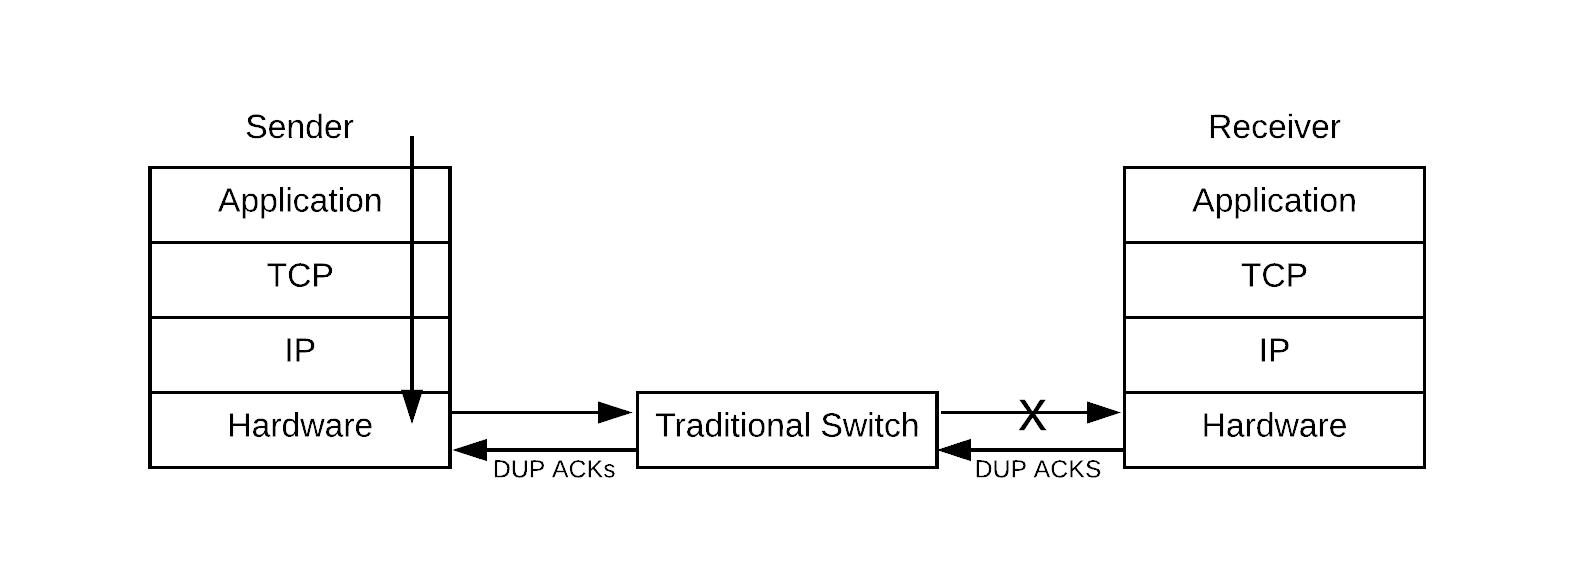
\includegraphics[width=\textwidth]{tradition-tcp.png}
	\caption{The standard convention of TCP handling.}
	\label{tradition-tcp}
\end{figure}

Currently, the DUP ACKs will traverse all the way back to the sender (\textbf{Figure \ref{tradition-tcp}}). The sender receives the DUP ACKs, then retransmits the packet with the next higher sequence number. 

\begin{figure}[h]
	\centering
	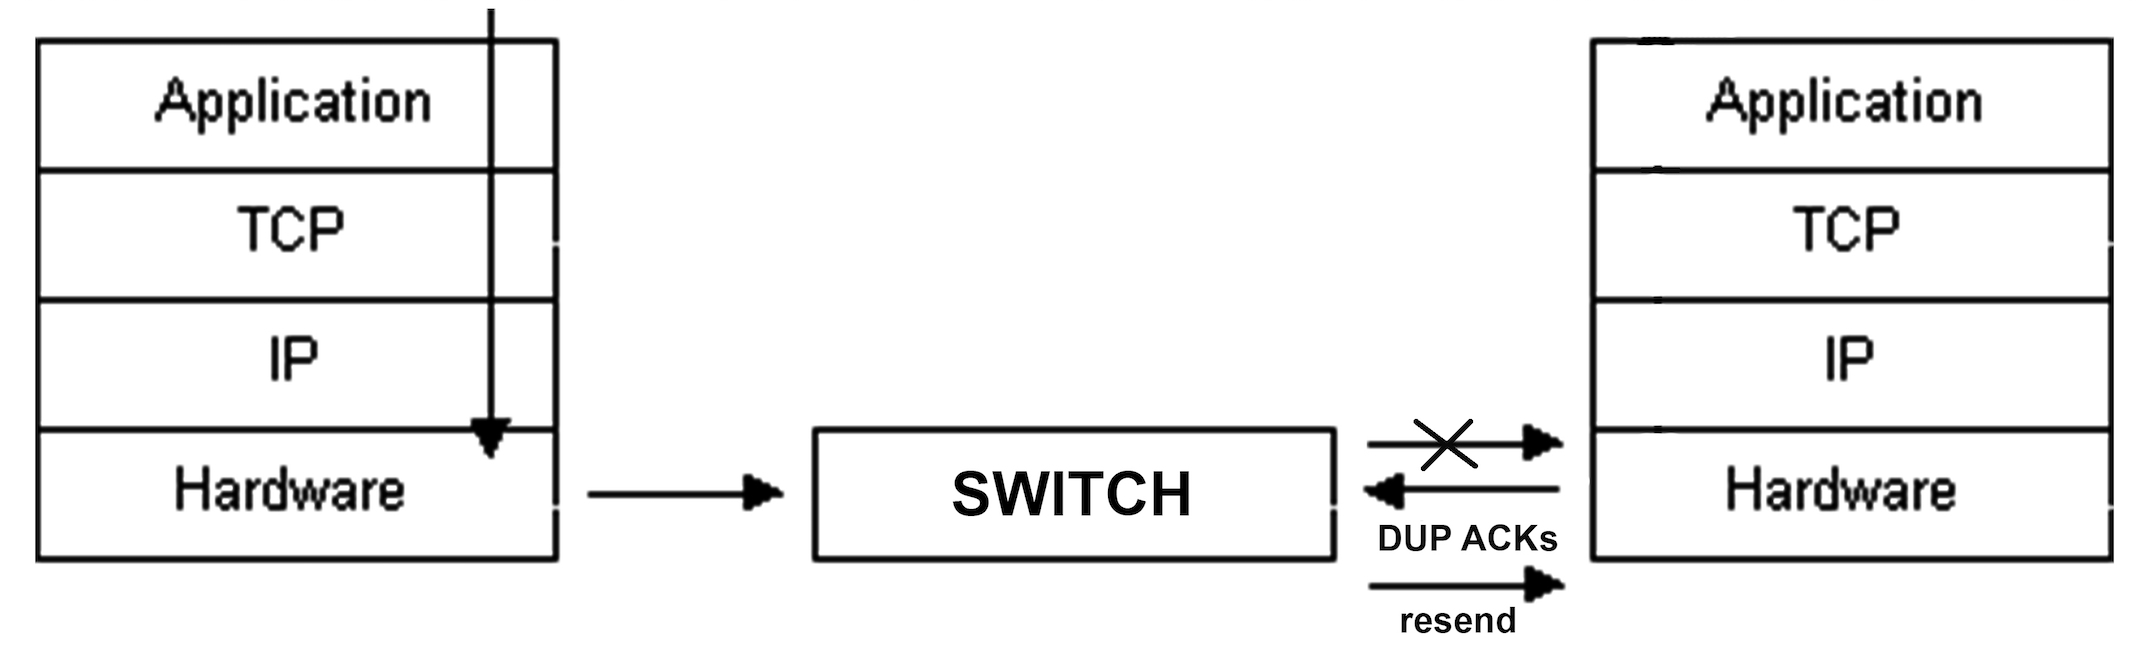
\includegraphics[width=\textwidth]{project-tcp.png}
	\caption{The proposed TCP handling.}
	\label{project-tcp}
\end{figure}

This project aims to design and implement a programmable switch that assists the TCP fast retransmit algorithm. The programmable switch will be able to retransmit the packets from within the network, instead of waiting for the DUP ACKs to get back to the host (\textbf{Figure \ref{project-tcp}}), thereby aims to reduce the response time to DUP ACKs and reduce unnecessary changes to the congestion window. The implementation will be based on the KVS concept, where the keys are the flow ID and the packet sequence number, and the value is the payload.

\section{Related Work}
	\subsection{TCP Congestion Control}
	One of the main aspects of TCP is congestion control, where a number of mechanisms are used to achieve high performance and avoid sending more data than the network is capable of forwarding, that is, to avoid causing network congestion. In particular, TCP uses a \textit{congestion avoidance} algorithm that includes various aspects of an additive increase/multiplicative decrease (AIMD) scheme, with other schemes such as \textit{slow start}, \textit{fast retransmit} and \textit{fast recovery} to achieve congestion avoidance. 
	
	The four intertwined algorithms are defined in more detail in RFC 5681\cite{rfc5681}. In this project, we are mostly interested in the \textit{fast retransmit} algorithm, which has been explained in the previous section.
	
	\subsection{Programmable Data Planes}
	The use of P4, netFPGA, etc.


\chapter{Preparation}
\textit{In this chapter, I first state the software I used and the starting point for this project. I move on to present the formal requirements. This is followed by a discussion of the different components of a programmable data plane, including the P4 programming language, the P4-SDNet compiler, the NetFPGA platform and the P4$\rightarrow$NetFPGA workflow. Finally, I discuss the project workflow.
}

\section{Software Used}
	Below I describe and justify, where necessary, the programming languages and development tools that I used.
	
	\subsection{Programming Languages}
	In this project, I used a multitude of languages, including \textbf{P4}, \textbf{Python}, \textbf{Verilog} and \textbf{Tcl}.
	
	\begin{itemize}
		\item \textbf{P4} is a language designed to describe packet processing logic in the packet forwarding planes. Besides, unlike general purpose languages such as C or Python, P4 is domain-specific with a number of constructs optimized around network data forwarding, hence is well-suited for implementing the forwarding plane of network elements such as our switch.
	
		\item \textbf{Python} was used extensively in the evaluation because of the \texttt{scapy} module, which enables the user to send, sniff, dissect and forge network packets. This capability allows me to write unit tests for my program by building customised packets, sending and checking them.
		
		\item \textbf{Verilog} was used to implement certain HDL modules within the P4-NetFPGA platform, in order to add or modify certain functionalities to suit the purpose of my design. It is the language of choice of the P4-NetFPGA platform.
		
		\item \textbf{Tcl} was used to write project wrappers and debug scripts.
	\end{itemize}

	I also made use of the \texttt{make} build automation tool to automate project builds, tests and benchmarks.
	
	\subsection{Development Tools}
	\begin{itemize}% [leftmargin=*] 0em: the starting letter is aligned, *: the dot is aligned.
		\item \textbf{The NetFPGA SUME Board}\footnote{A collaborative effort between Digilent, the University of Cambridge and Stanford University.} is an advanced board that features one of the largest and most complex FPGA’s ever produced, a Xilinx Virtex-7 690T supporting thirty 13.1 GHz GTH transceivers. This board easily supports simultaneous wire-speed processing on the four 10Gb/s Ethernet ports, and it can manipulate and process data on-board, or stream it over the 8x Gen3 PCIe interface and the expansion interfaces. It is indeed ideal for any high-performance design such as in this project.
					
		\item \textbf{P4$\rightarrow$NetFPGA} (P4 on NetFPGA) is the environment to develop and test P4 programs using the Xilinx P4-SDNet\footnote{\url{https://www.xilinx.com/products/design-tools/software-zone/sdnet.html}} toolchain within the NetFPGA SUME reference switch design.
		
		\item \textbf{Vivado$^{\textrm{\textregistered}}$ Design Suite} is a software suite produced by Xilinx\footnote{\url{https://www.xilinx.com/}} for synthesis and analysis of HDL designs. Vivado was used in the project because it is the design environment for FPGA products from Xilinx, and is tightly-coupled to the architecture of such chips. Its flexibility also enables me to simulate my design behaviour with different stimuli, synthesize the design to hardware and perform timing analysis.
		
		\item \textbf{Git} was used for version control, allowing quick roll-back and efficient management of multiple source trees using branches to implement different functionalities at various stages of the project.
	
		\item \textbf{Backups} were taken by uploading relevant files to Microsoft OneDrive\footnote{\url{https://onedrive.live.com/about/en-gb/}}. The git repository itself was hosted remotely on GitHub\footnote{\url{https://github.com/ttbui11/part-ii-proj/}}.
	\end{itemize}

\section{Starting Point} 
\label{sec:start}
	This project uses the knowledge about TCP introduced in the Part IB \textit{Computer Networking} course and the experience in Electronic Computer-aided Design (ECAD) and working with a design-flow for Field Programmable Gate Arrays (FPGAs) from Part IB \textit{ECAD and Architecture Practical Classes}.
	
	During the development of this project, I acquired further knowledge from the materials covered in the following Part II and Part III courses:%
	
	\begin{itemize}
		\item \textit{High Performance Networking} --- Introduction to P4 and P4$\rightarrow$NetFPGA;%
		\item \textit{Principle of Communications} --- TCP flow control and congestion control. Design choices for scheduling and queue management algorithms for packet forwarding;%
		\item \textit{\LaTeX \ and MATLAB} --- Typesetting the project proposal and dissertation.%
	\end{itemize}
	
	In terms of familiarity, I had no prior experience with P4 programming language, the P4$\rightarrow$NetFPGA workflow and Tcl, and little experience with Verilog, based on the similar language SystemVerilog learnt in Part IB \textit{ECAD and Architecture Practical Classes}. Therefore, I had to spent some time learning the languages and the workflow. I had some prior experience in Python and Git from various projects and internships.
	
	The main code in P4 and the tests in Python were written from scratch, using the template given by the P4$\rightarrow$NetFPGA workflow as the starting point. The code for the additional modules and externs in Verilog as well as the project wrappers in Tcl are modified from some of the current modules to suit the required functionalities.
	
\section{Requirements Analysis}
This project has one software deliverable: an implementation of a programmable switch that will retransmit a packet when it receives the third DUP ACK from the receiver.

Below is a list of requirements and extensions for the deliverable, prioritised using \textit{MoSCoW} criteria \cite{moscow}:

\textbf{Must have}
\begin{itemize}
	\item Have an implementation of the switch in P4. 
	\item The implementation works correctly in an SDNet simulation.
	\item The implementation works correctly in a SUME simulation.
	\item The implementation works correctly in a hardware simulation.
	\item A performance evaluation of the design.
\end{itemize}

\textbf{Should have}
\begin{itemize}
	\item The switch will send a notification to the source if the retransmit fails.
	\item A performance evaluation in comparison to existing TCP fast retransmit mechanism.
\end{itemize}

\textbf{Could have}
\begin{itemize}
	\item The design will support more than a single flow, and support the configuration of flows to monitor.
	\item The design will support different packet sizes.
	\item The design has the ability to adaptively add or remove flows to monitor.
\end{itemize}

\textbf{Won't have}
\begin{itemize}
	\item The implementation will not be simulated using network simulators such as ns2 or omnet++.
\end{itemize}

\section{The P4 Language}
P4 (Programming Protocol-independent Packet Processors) has become the \textit{de facto} standard language for describing how network packets should be processed, and is becoming widely used by many developers in  conjunction with SDN control protocols like OpenFlow. This section gives a brief overview of the P4 programming language with the aim to provide sufficient basis of the project.

Many targets implement both a control plane and a data plane. P4 is designed to specify only the data plane functionality of the target. P4 programs also partially define the interface by which the control plane and the data plane communicate, but P4 itself cannot be used to describe the control plane functionality of the target. Thus, in the remaining of this dissertation, when we refer to P4 as “programming a target”, we mean “programming the data plane of a target”. Figure \ref{p4target} describes the canonical process of programming a P4 target. The vendor of a packet processing device provides three components to the user:

\begin{itemize}
	\item The packet processing target device.
	\item A P4 architecture model to expose the programmable features of the target to the programmer.
	\item A compiler to map the user’s P4 program into a target-specific configuration binary file which is used to tell the target how it should be configured to process packets.
\end{itemize}

The programmer will write a P4 program to instantiate the architecture model, by filling its programmable components. The programmer also provides control software (i.e. a control plane) which is responsible for controlling the packet processing device at run time.

\begin{figure}[!ht]
	\centering
	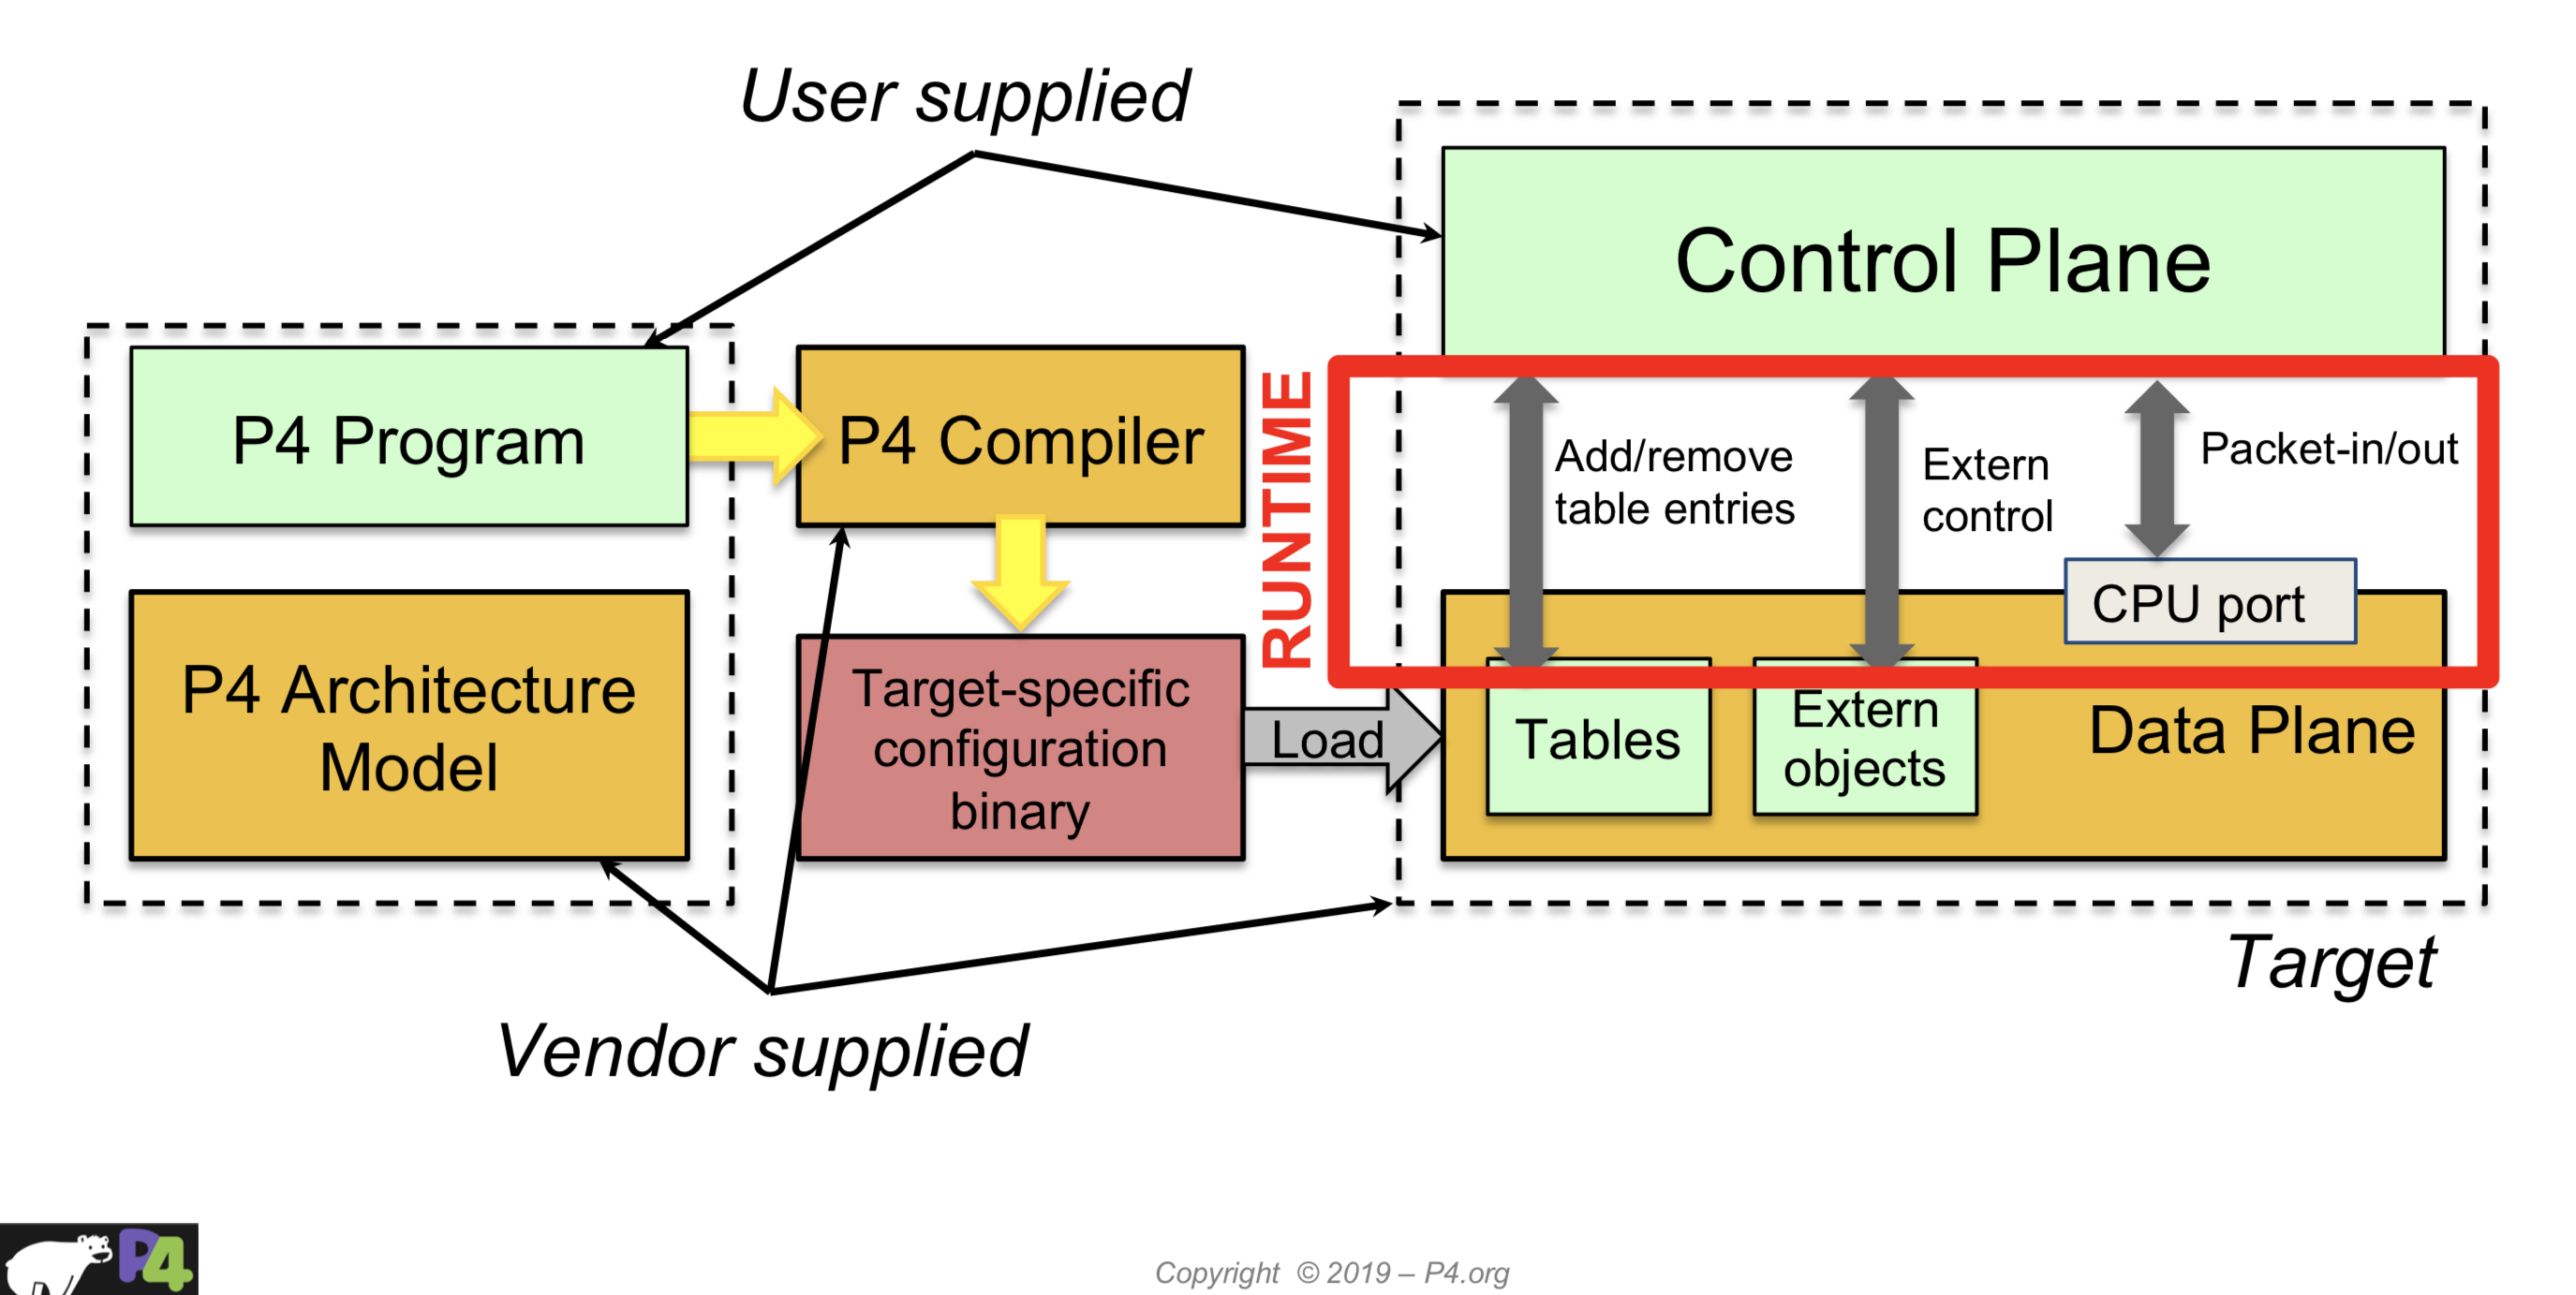
\includegraphics[width=\textwidth]{p4target.png}
	\caption{The process of programming a P4 target. Source: \href{https://p4.org}{P4.org -- Copyright \textcopyright\ 2019}.} 
	\label{p4target}
\end{figure}

In order to make the devices ``protocol-independent'', i.e. without built-in implementations of specific protocols, P4 allows us to define the format of all protocol headers that we want the device to handle using the \texttt{header} keyword. Here is an example that shows the definition of the Ethernet header in the project. The IPv4 and TCP headers are defined similarly. Note that \texttt{typedef} statements can also be used to make the code more readable.

{\renewcommand{\baselinestretch}{0.8}\small
	\begin{verbatim}
    typedef bit <48> EthAddr_t;

    header Ethernet_h {
      EthAddr_t dstAddr;
      EthAddr_t srcAddr;
      bit<16> etherType;
    }
    
    header IPv4_h {
      bit<4> version;
      ...
    }
    
    header TCP_h {
      bit<16> srcPort;
      ...
    }
    
   	struct Parsed_packet {
  	  Ethernet_h ethernet;
  	  IPv4_h ip;
  	  TCP_h tcp;
   	}
	\end{verbatim}
}

This makes P4-programmable switch differ from a traditional switch in two fundamental ways:
\begin{itemize}
	\item The data plane functionality is defined by the P4 programmer, rather than by the manufacturer of the switch. The data plane is configured at initialisation time to implement the functionality described by the P4 program and has no built-in knowledge of existing network protocols.
	\item The set of tables and other objects in the data plane are no longer fixed, but defined by the P4 program. The P4 compiler then generates the API that the control plane uses to communicate with the data plane, using the same channels as in a fixed-function device.
\end{itemize}

In this project, we will be using the P4-SDNet compiler (``the compiler''), the NetFPGA SUME board (``the target device''), and the SimpleSumeSwitch architecture of the P4$\rightarrow$NetFPGA workflow (``the architecture model''), all of which will be described in more detail in the next three sections.

\section{The Xilinx P4-SDNet}
The Xilinx P4-SDNet compiler is the centerpiece of the P4$\rightarrow$NetFPGA workflow. It is the Xilinx SDNet original design environment for an internally-created packet processing language called PX \cite{px}, with a P4 to PX translator. Figure \ref{sdnet} depicts the process of compiling P4 programs that target the SimpleSumeSwitch architecture using P4-SDNet. The front end translator maps P4 programs into corresponding PX programs and also produces a JSON file with information about the design that is required by the runtime control software. The PX program is passed, along with configuration parameters, into SDNet which then produces an HDL module that implements the user’s P4 program, and has standard AXI-Stream packet interfaces and an AXI-Lite control interface. SDNet generated designs can be configured to process packets at line rates between 1 and 400 Gb/s, hence is able to easily handle the aggregate 40G rate in the SUME reference switch design. SDNet also produces a SystemVerilog simulation testbench, C drivers to configure the PX tables, and an optional C++ model of the PX program to be used for debugging purposes.

\begin{figure}[!h]
	\centering
	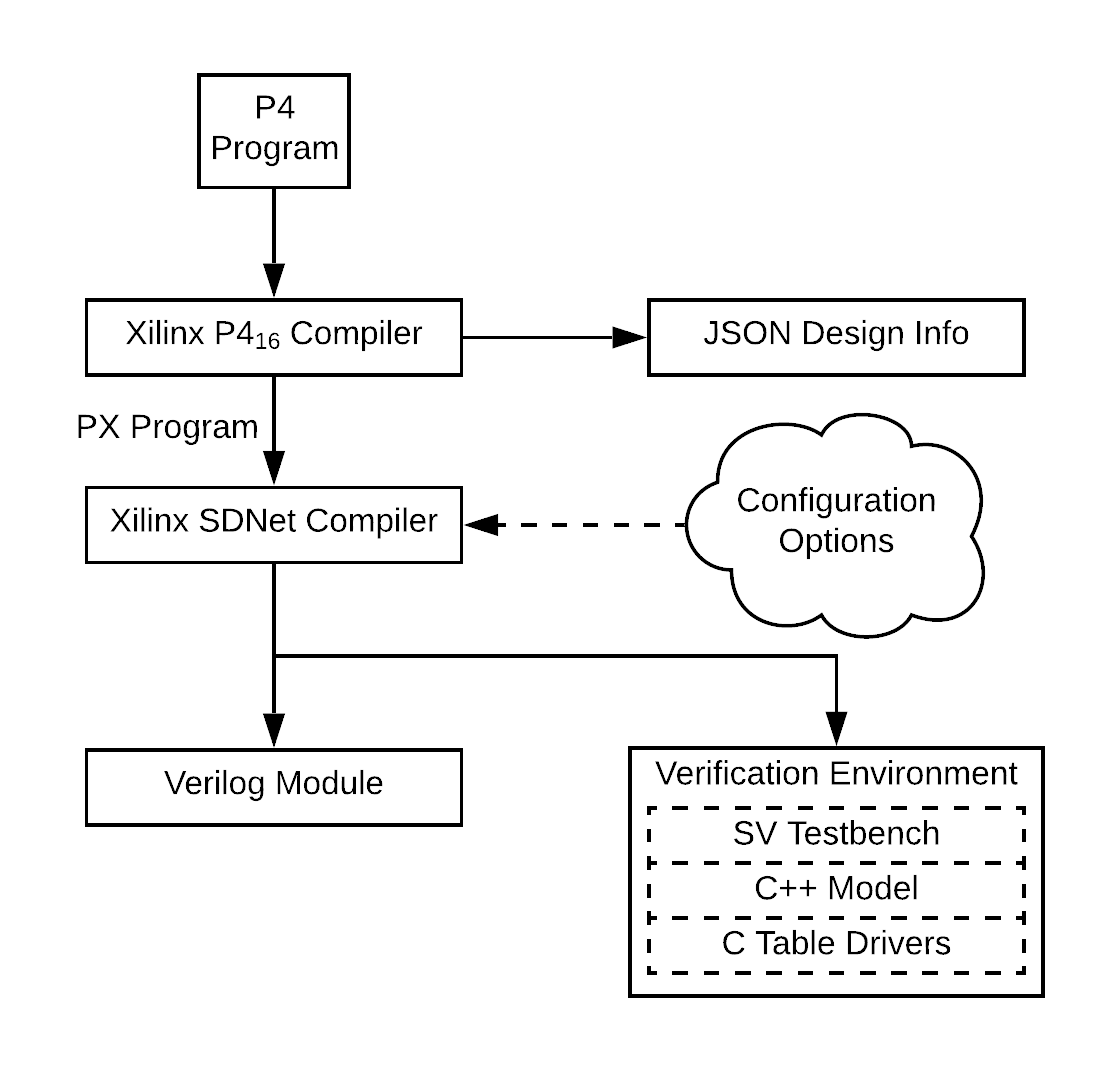
\includegraphics[width=0.7\textwidth]{sdnet.png}
	\caption{The Xilinx P4-SDNet compilation flow. P4 programs are first translated into a PX program, which is then compiled into a Verilog module using the SDNet flow. SDNet also produces a verification environment.}
	\label{sdnet}
\end{figure}

\section{The NetFPGA Platform}
The NetFPGA (Networked FPGA) project is a teaching and research tool designed to allow packets to be processed at line-rate in programmable hard-ware. It consists of four components: boards, tools and reference designs, a community of developers and contributed projects. The SUME board that was used in this project, which has total I/O capacity of 100 Gb/s, is the latest product in the NetFPGA hardware family. 

Figure \ref{ref-switch} depicts a block diagram of the canonical NetFPGA reference design which is used for switches, NICs, and IPv4 routers. It consists of four 10G SFP+ input/output ports along with one DMA interface for the CPU path. The NetFPGA data path consists of three main components: Input Arbiter, Output Port Lookup, and Output Queues. The Input Arbiter admits packets from the ports into the data path, towards the Output Port Lookup Module, where the main packet processing occurs and an output port is selected. The Output Queues buffer packets while they wait to be sent to the outputs. The core data path uses a 256-bit wide bus and runs sufficiently fast at 200 MHz to support an aggregate of 40 Gb/s from all four SFP+ ports.

The limitation of this platform is that it requires a substantial knowledge in both hardware design and networking, with programs written in Verilog or VHDL. To overcome this, the P4$\rightarrow$NetFPGA workflow was created to make it much easier to process packets in hardware and prototype new systems without being bogged down in hardware development.

\begin{figure}[!ht]
	\centering
	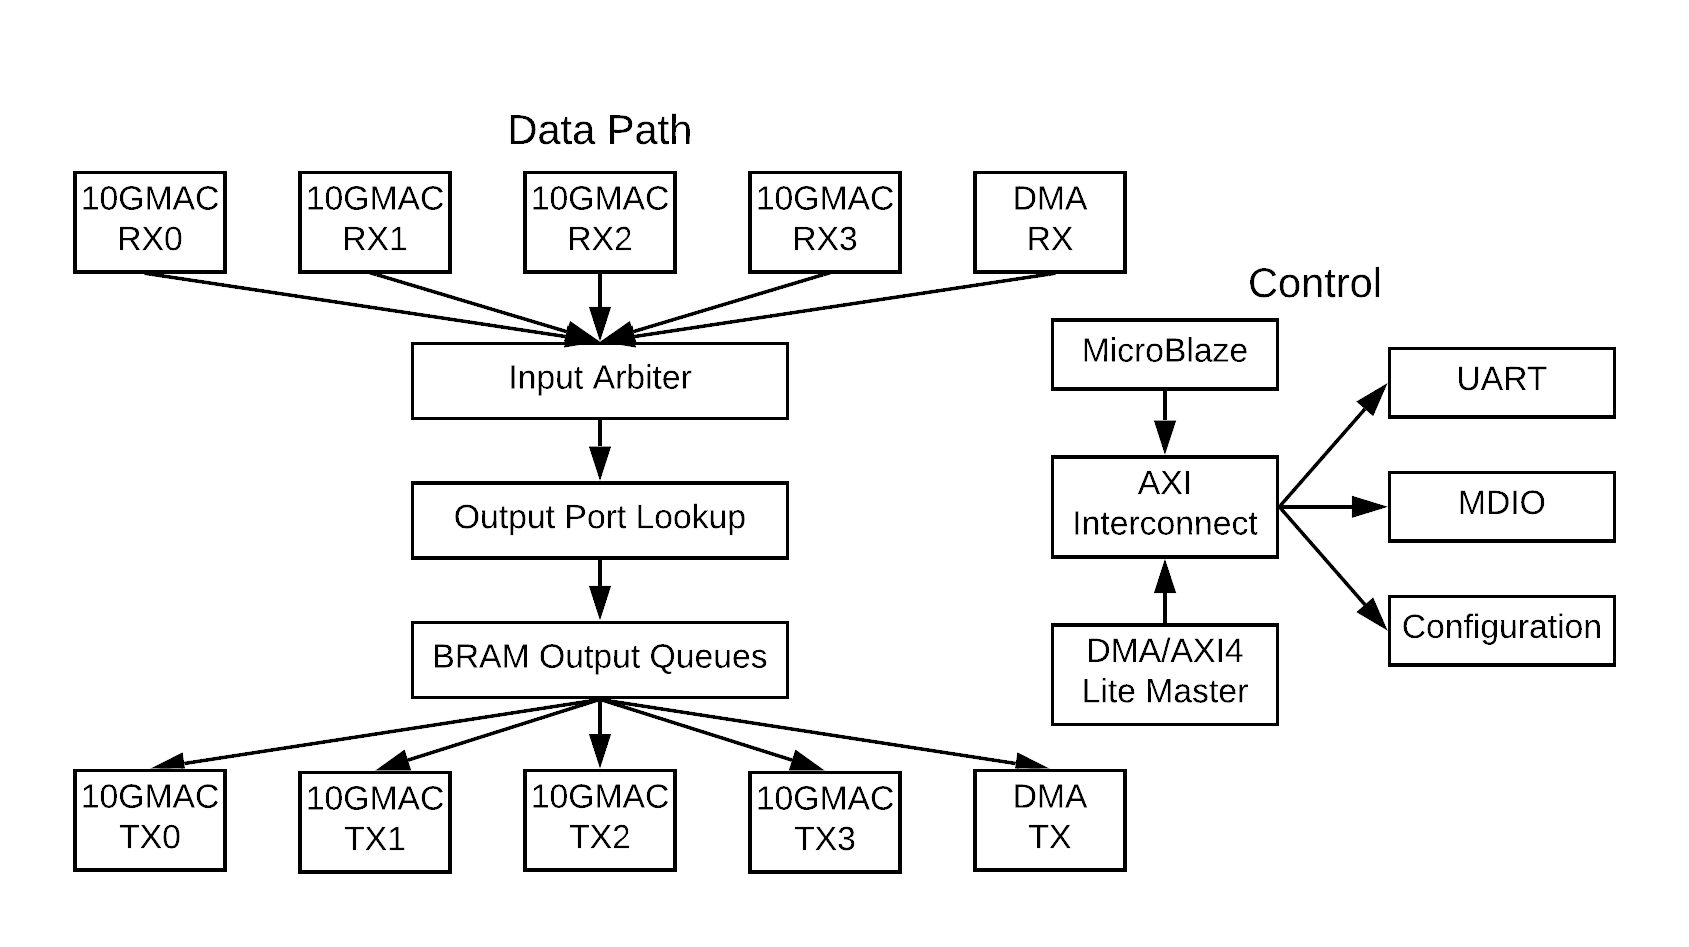
\includegraphics[width=\textwidth]{ref-switch.png}
	\caption{Block diagram of the NetFPGA reference design.}
	\label{ref-switch}
\end{figure}

\section{The P4$\rightarrow$NetFPGA Workflow}
The \textit{SimpleSumeSwitch} (SSS) is the P4 architecture that is currently defined for the NetFPGA SUME board. The architecture consists of a single parser, a single match-action pipeline, and a single deparser, as shown in Figure \ref{sss}. The SSS is a great architecture because it is simple and easy to understand, yet remains flexible enough to allow developers to implement a variety of different networking protocols and algorithms. 

The SimpleSumeSwitch’s \verb|sume_metadata| bus corresponds to the tuser bus in the SUME reference switch design, and is defined as follows:

{\renewcommand{\baselinestretch}{0.8}\small
	\begin{verbatim}
    struct sume_metadata_t {
        bit<16> dma_q_size;     // measured in 32-byte words
        bit<16> nf3_q_size;     // measured in 32-byte words
        bit<16> nf2_q_size;     // measured in 32-byte words
        bit<16> nf1_q_size;     // measured in 32-byte words
        bit<16> nf0_q_size;     // measured in 32-byte words
        bit<8> send_dig_to_cpu; // send digest_data to CPU
        port_t dst_port;        // one-hot encoded (see below)
        port_t src_port;        // one-hot encoded (see below)
        bit<16> pkt_len;        // (bytes) unsigned int
    }
	\end{verbatim}
}

where the format of the \verb|dst_port| and \verb|src_port| fields is:

{\renewcommand{\baselinestretch}{0.8}\small
\begin{verbatim}
  bit-7     bit-6     bit-5     bit-4     bit-3     bit-2     bit-1     bit-0
(nf3_dma)-(nf3_phy)-(nf2_dma)-(nf2_phy)-(nf1_dma)-(nf1_phy)-(nf0_dma)-(nf0_phy)
\end{verbatim}
}

and the functionality of each field is described by Table \ref{sume}. 

\begin{figure}[!ht]
	\centering
	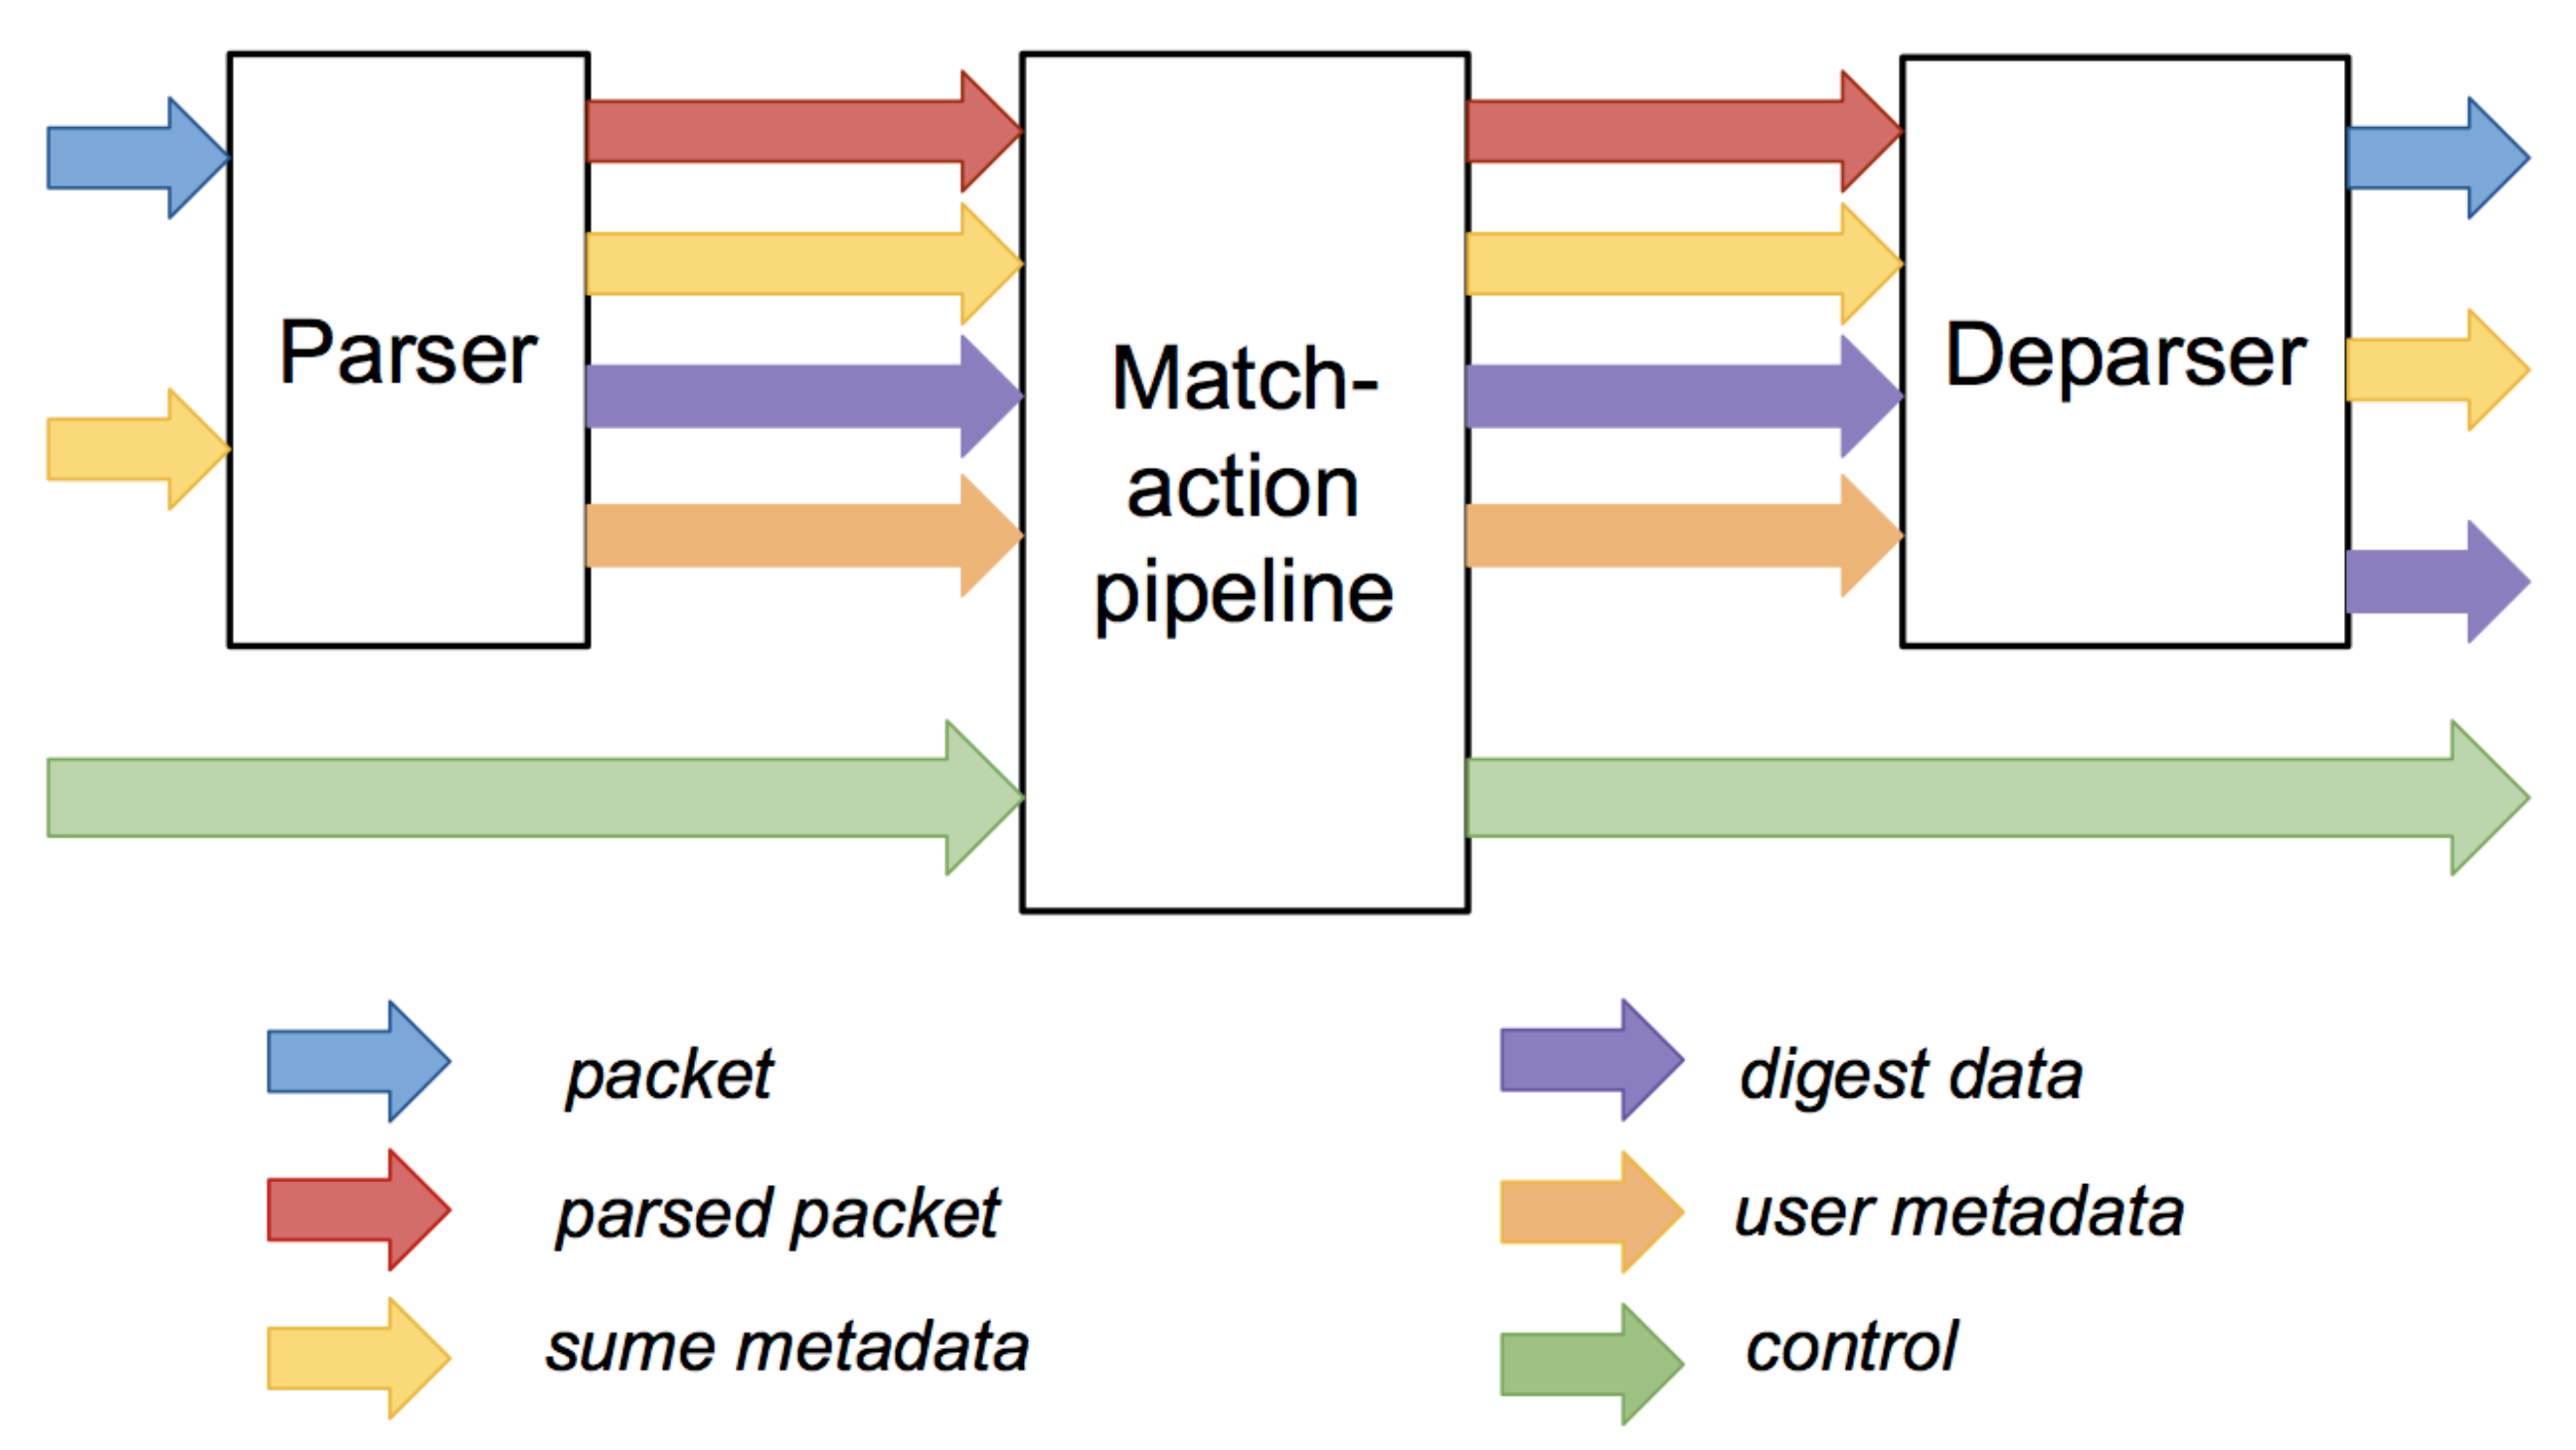
\includegraphics[width=0.9\textwidth]{sss.png}
	\caption{Block diagram of the SimpleSumeSwitch P4 architecture used within the P4$\rightarrow$NetFPGA workflow. Source: \href{https://github.com/NetFPGA/P4-NetFPGA-public/wiki/Workflow-Overview\#simplesumeswitch-architecture}{P4$\rightarrow$NetFPGA Home Wiki}.} 
	\label{sss}
\end{figure}

\begin{table}[!ht]
	\begin{center}
		\caption{Description of the SimpleSumeSwitch \texttt{sume\_metadata} fields.}
		\label{sume}
		\begin{tabular}{ | c | c | p{10cm} |}
			\hline
			\textbf{Field Name} & \textbf{Size (bits)} & \multicolumn{1}{>{\centering\arraybackslash}m{10cm}|}{\textbf{Description}} \\ \hline
			\texttt{pkt\_len}  & 16 & Size of the packet in bytes (not including the Ethernet preamble or FCS) \\ \hline
			\texttt{src\_port} & 8 & Port on which the packet arrived (one-hot encoded) \\ \hline
			\texttt{dst\_port} & 8 & Set by the P4 program -- which port(s) the packet should be sent out of (one-hot encoded) \\ \hline
			\texttt{send\_dig\_to\_cpu} & 8 & Set the least significant bit of this field to send the \texttt{digest\_data} to the CPU \\ \hline
			\texttt{*\_q\_size} & 16 & Size of each output queue at P4 processing start time, measured in 32-byte words \\ \hline
		\end{tabular}
	\end{center}
\end{table}

Figure \ref{p4-netfpga} outlines the automated P4$\rightarrow$NetFPGA workflow. We first write a P4 program which is compiled (by Xilinx P4-SDNet) into an HDL instance of the SSS architecture. The SSS module is then automatically integrated into the NetFPGA reference switch design by replacing the default Output Port Lookup module. The flexibility of the SSS architecture means that it could also be extended or completely replaced by writing a new architectural model. For this project, I will modify the NetFPGA Reference Switch Pipeline to include a Cache Queue that will buffer packets. Section \ref{sec:arch-design} will explain the customised architecture in more detail.

To sum up, the P4$\rightarrow$NetFPGA workflow includes the following steps:
\begin{enumerate}[label=(\arabic*)]
	\item Write P4 program.
	\item Implement custom extern modules, if any.
	\item Write Python scripts to generate test data for SDNet simulations.
	\item Run HDL simulations.
	\item Build bitstream for FPGA.
	\item Test the design on hardware.
\end{enumerate}

\begin{figure}[!ht]
	\centering
	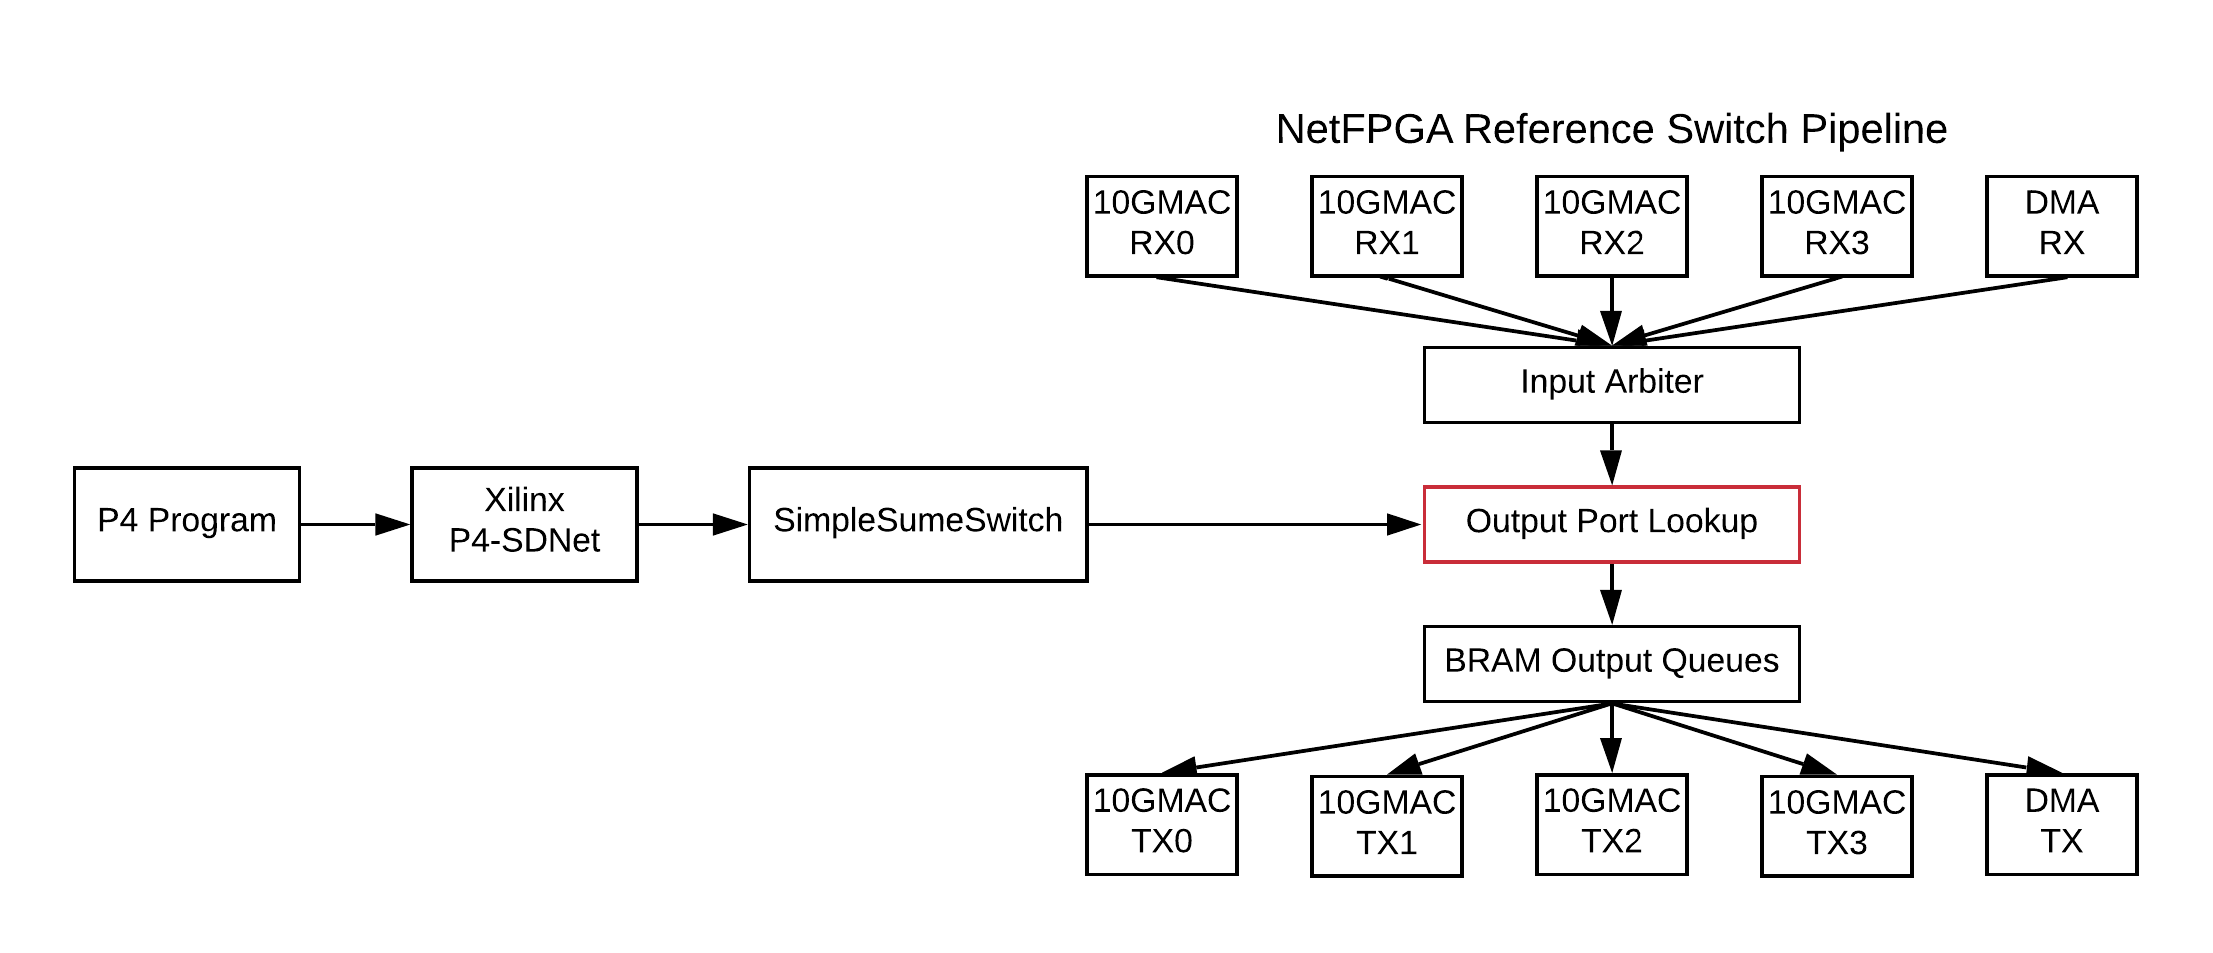
\includegraphics[width=\textwidth]{p4-netfpga.png}
	\caption{The automated P4$\rightarrow$NetFPGA compilation flow. P4 programs are compiled into an HDL instance of the SimpleSumeSwitch architecture, which is then used to replace the Output Port Lookup module in the NetFPGA Reference Switch Design.}
	\label{p4-netfpga}
\end{figure}

\section{Project Workflow}
	\subsection{Preparation Stage}
	I spent the first two weeks of the project learning the P4 language, setting up the development environment and learning the P4$\rightarrow$NetFPGA workflow.
	
	The P4 Language Consortium \cite{p4.org} provides a set of exercises to get me started. I completed their tutorial\footnote{\url{https://github.com/p4lang/tutorials}}, from which I learned the language basics such as basic forwarding and basic tunnelling. I also learned to use P4 tables and actions to implement advanced behaviour such as source routing and load balancing. 
	
	Most of the time spent in setting up the NetFPGA environment went into getting approval for access to the live development repositories, including the P4$\rightarrow$NetFPGA and the NetFPGA-SUME codebase, and various licenses and tools necessary to use the P4$\rightarrow$NetFPGA toolchain (Xilinx P4-SDNet and Vivado Design Suite). Where appropriate, the licenses are quoted at the beginning of the file. The NetFPGA SUME board was already installed and configured, and is connected to a machine with the appropriate system requirements and dependencies located in the Computer Laboratory. To access the board from my personal device, I set up a Virtual Private Network (VPN) and \texttt{ssh} to the machine.
	
	Finally, I learned the P4$\rightarrow$NetFPGA workflow through a series of exercises, provided by the NetFPGA Github Organisation\footnote{\url{https://github.com/NetFPGA}}. The workflow provides a template for a general P4 program following the SSS architecture model, from which I will start to write my implementation, as stated in Section \ref{sec:start}. The main challenge of this part is learning Verilog and Tcl in a short amount of time.
	
	\subsection{Architecture Design Stage}
	\label{sec:arch-design}
	Following the preparation stage, I designed the architecture of the switch. I would then write P4 programs that follow the architecture and make adjustments to the design where necessary.
		
	\subsubsection{Network Level}
	The switch will embed the TCP fast retransmit mechanism and will be one hop away from the receiver, as illustrated in Figure \ref{fig:network}. Since the switch is programmable, it will be configured to buffer only packets of particular applications, identified by their flow number, while transmitting other packets normally. This design avoids introducing unnecessary buffering of packets of other flows which is the cause of bufferbloat.
	\begin{figure}[!hb]
		\centering
		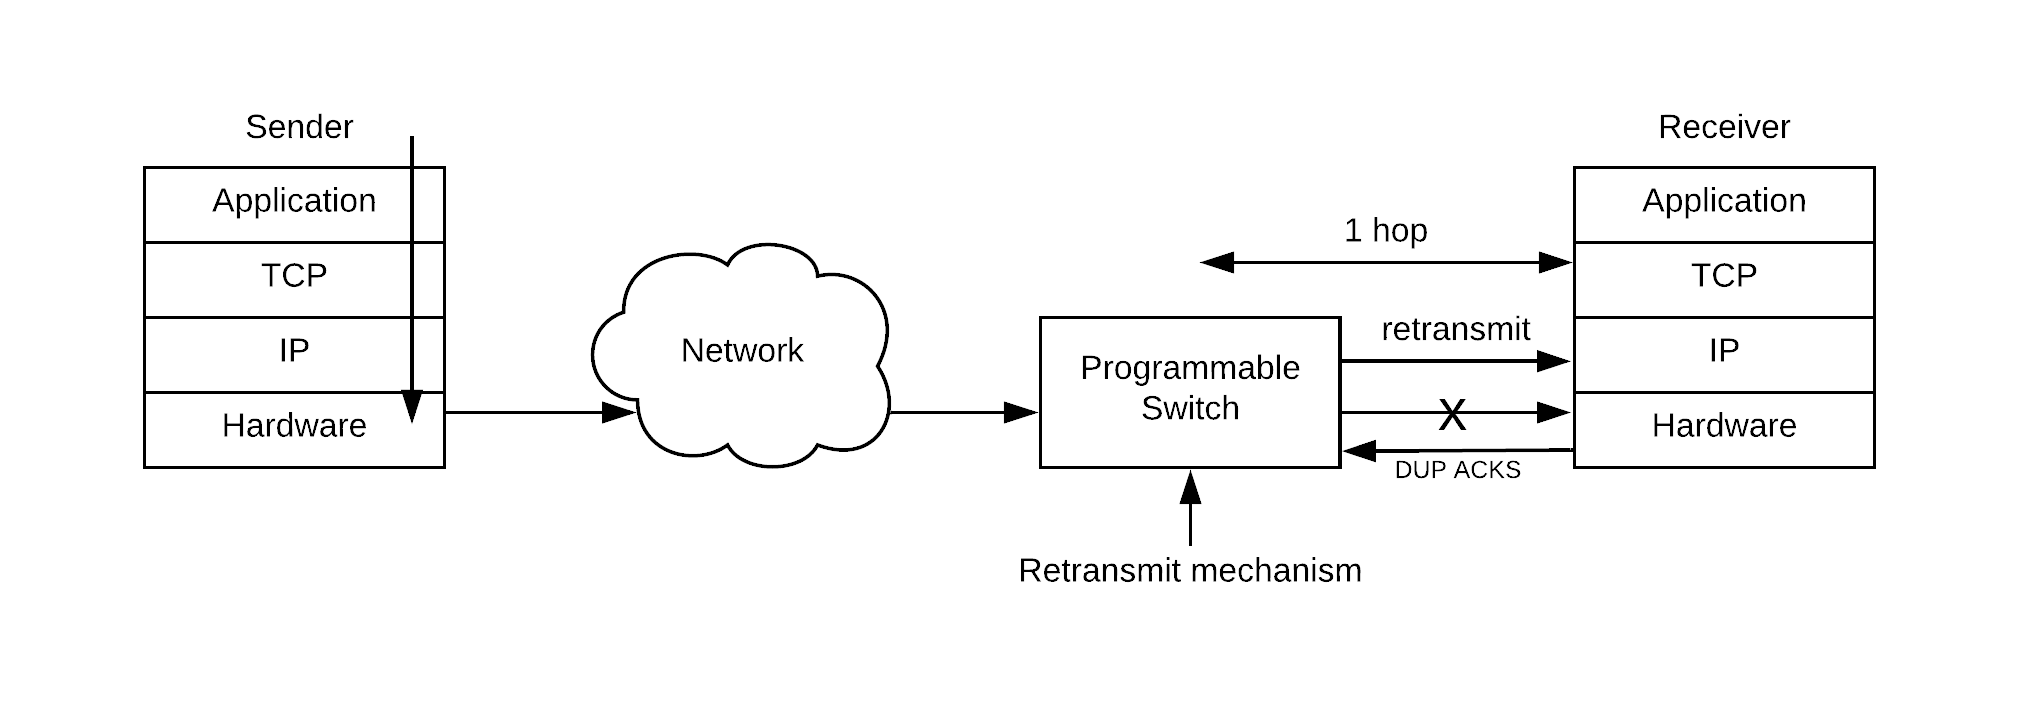
\includegraphics[width=\textwidth]{network.png}
		\caption{The network.}
		\label{fig:network}
	\end{figure}

	\subsubsection{System Level}
	The first design uses a hash table to map flow number to another hash table with the packet sequence number as the key and the packet itself as the value. The flowchart showing the buffering logic of this design is given in Figure \ref{fig:flowchart}. However, this design does not work due to the limitations of SDNet and the SSS architecture of the NetFPGA platform. The SSS architecture only supports programmable packet processing, i.e. operations on packet headers only. This means that the P4 program would not be able to access the packet payload to store it in the second hash table. Hence, this design cannot be fully expressed in P4 alone.
	
	\begin{landscape}
		\begin{figure}[!ht]
			\centering
			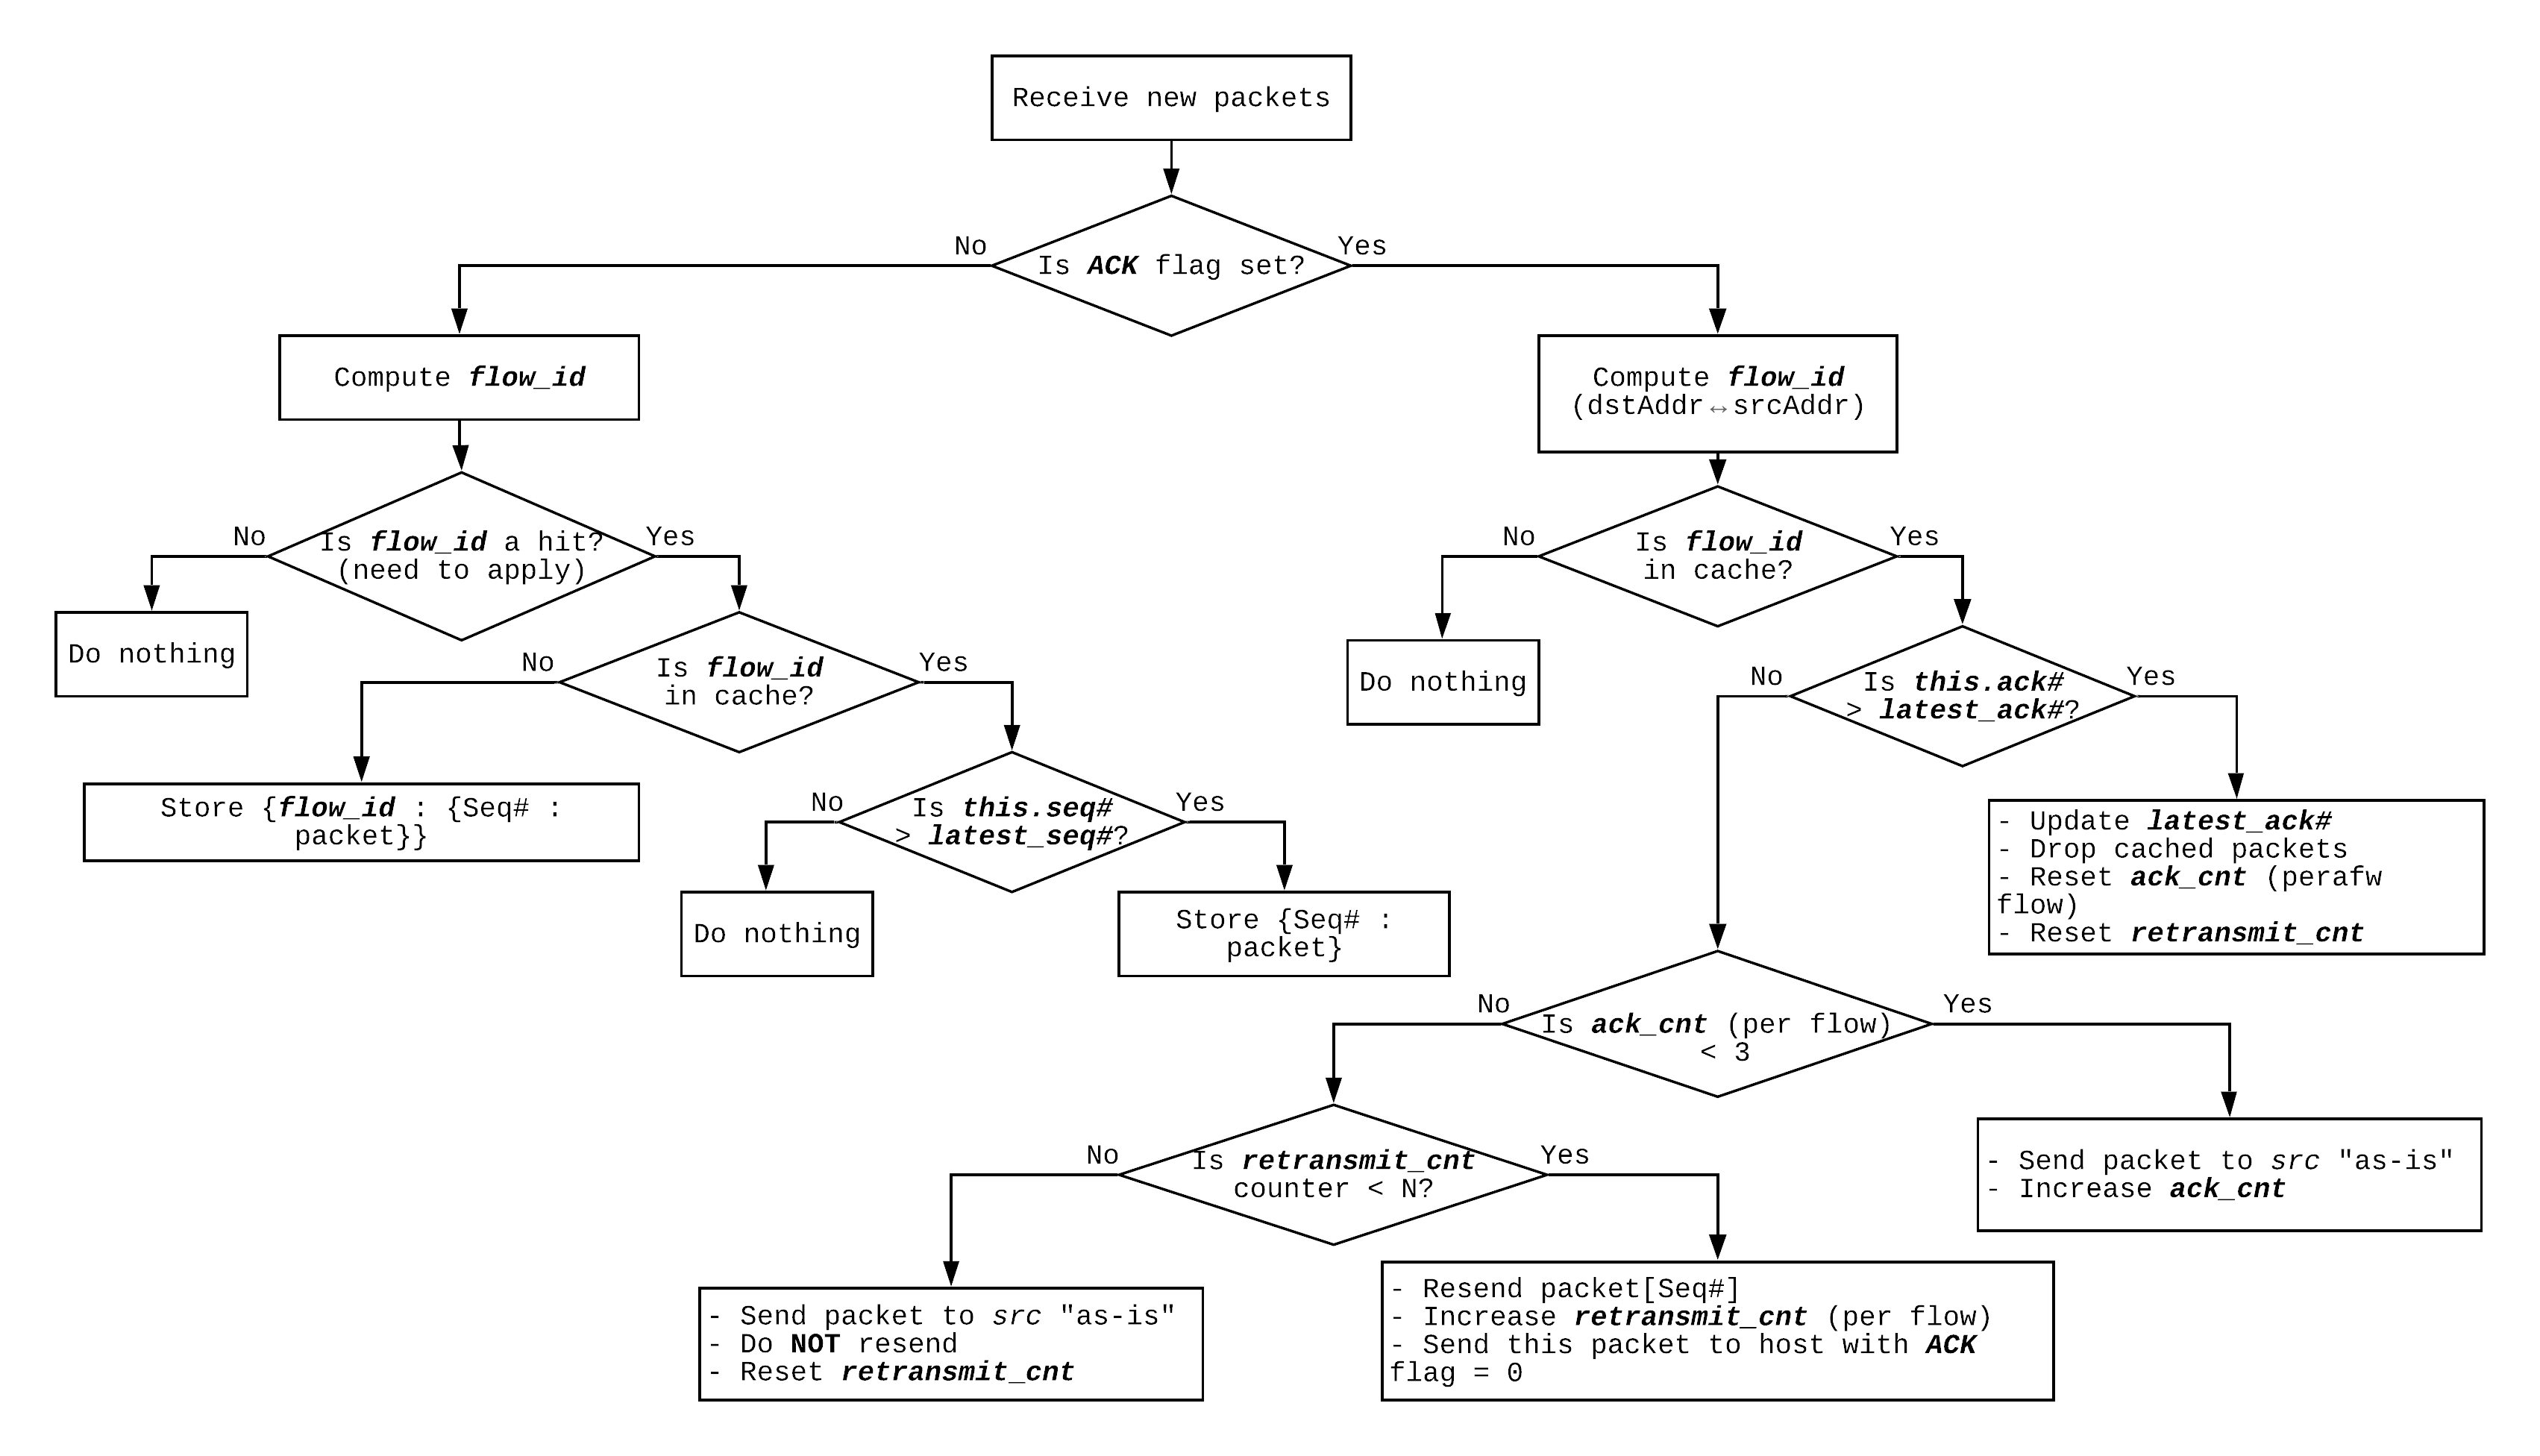
\includegraphics[width=1.5\textwidth]{flowchart.png}
			\caption{Flowchart shows the packet buffering logic of the first design.}
			\label{fig:flowchart}
		\end{figure}
	\end{landscape}
	
	After careful study of the first design and the platform, I decided to add an additional HDL module that follows the SSS module in the NetFPGA reference switch pipeline. The additional HDL module is called the Cache Queue and it will buffer packets to be retransmitted. Our reference switch pipeline will now look like Figure \ref{fig:modified-design}. In this pipeline, when a packet exits the SSS module, it will be duplicated and buffered in both the output queue and the cache queue. While the output queue sends the packet to the output ports as soon as it can, the cache queue will hold on to the packet. Once there is a ``signal'' from another packet, the cache queue will drop or send the packet to the output accordingly. The role of the Output Arbiter is similar to that of the Input Arbiter---merging multiple input streams into one output stream---albeit having different names. Section \ref{sec:cachequeue} will explain the implementations of both the Cache Queue and the Output Arbiter in more detail.
	
	\begin{figure}[!ht]
		\centering
		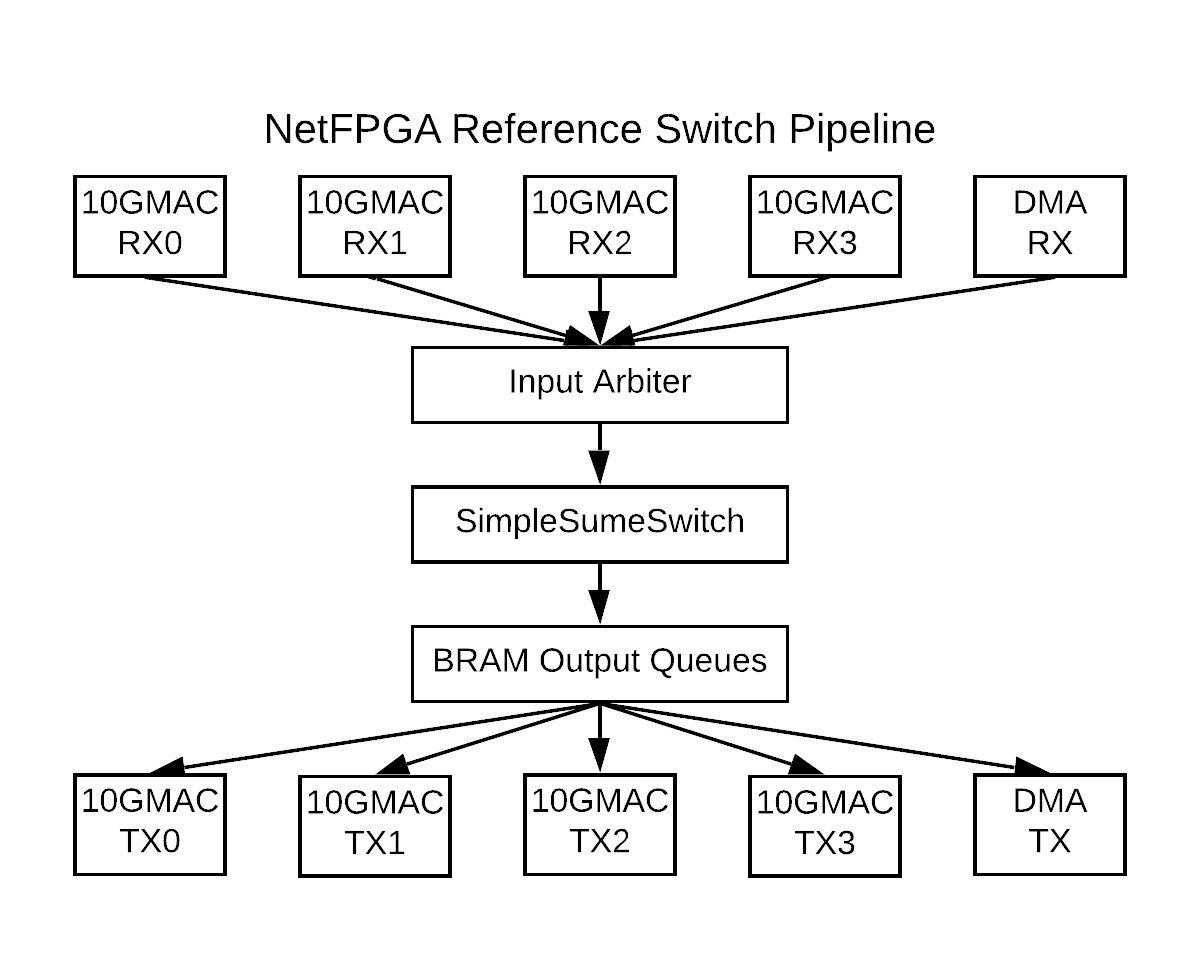
\includegraphics[width=0.75\textwidth]{netfpga-ref-switch.png}
		\caption{Block diagram of the NetFPGA reference switch design.}
		\label{fig:netfpga-ref-switch}
	\end{figure}
	
	\begin{figure}[!ht]
		\centering
		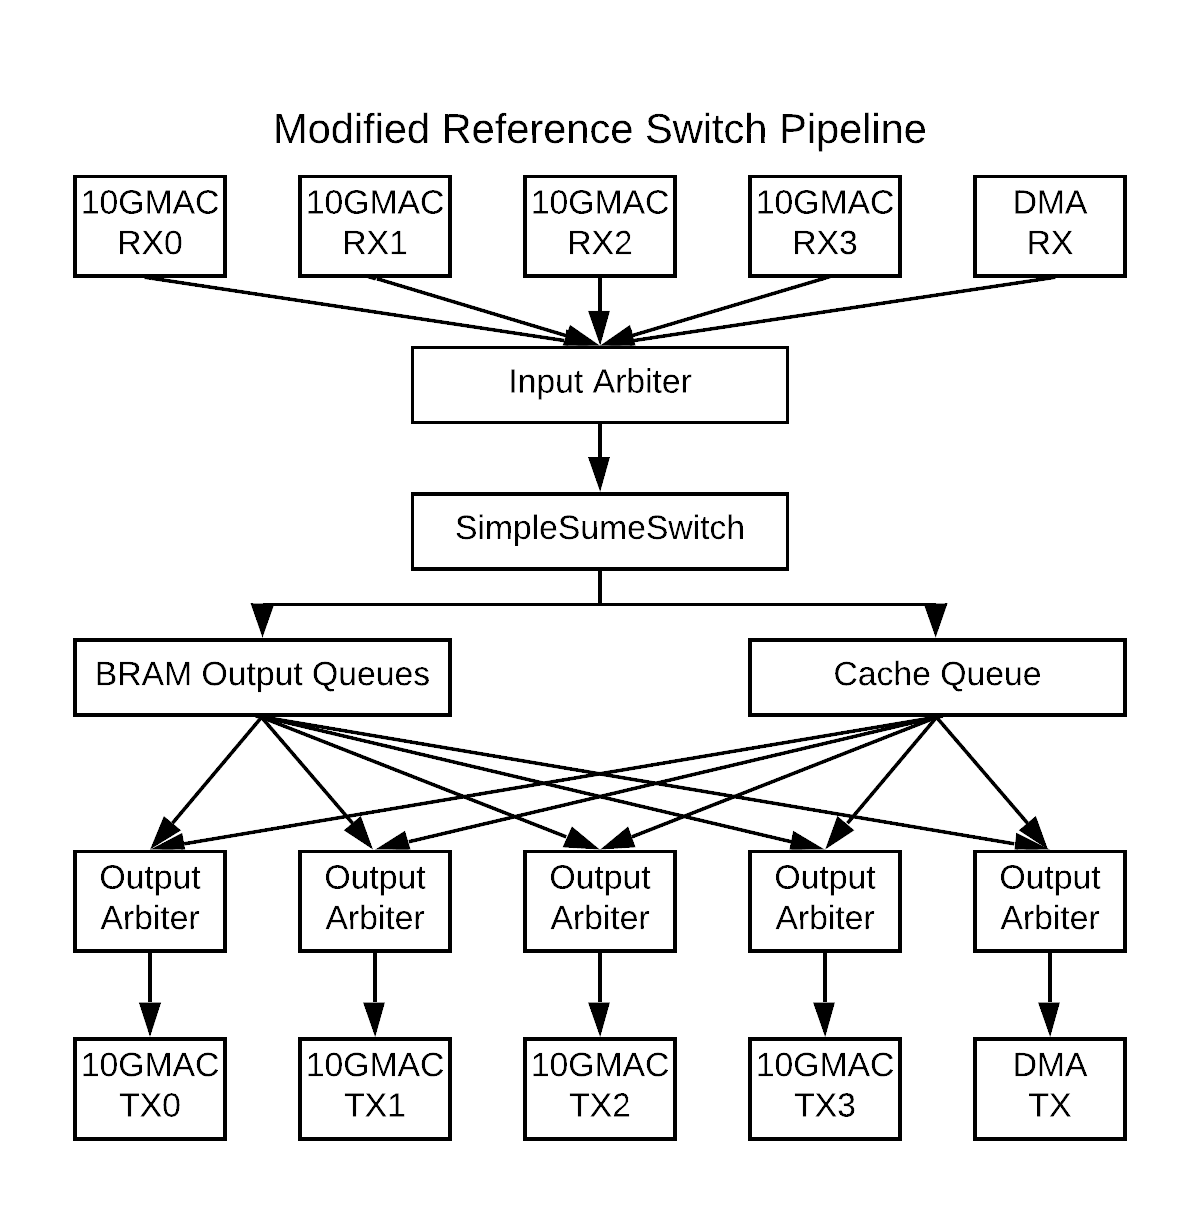
\includegraphics[width=0.6\textwidth]{modified-design.png}
		\caption{Block diagram of the modified reference switch pipeline. Packets are duplicated after the SSS module and being buffered in the Cache Queue.}
		\label{fig:modified-design}
	\end{figure}
		
	\subsection{Implementation Stage}
	
	In order to fulfil the requirements analysis, I follow the \textit{spiral development model} \cite{spiral} with an iteration count equal to the number of major functionalities to add. This allows for continual implementation, testing and integration of the different functionalities. Figure \ref{fig:workflow} shows the workflow of the implementation stage of this project. After laying out the requirements and designing the architecture, I will start to write the implementation in P4 and test it by running an SDNet simulation, which is written in Python. Then, I will code the HDL modules and configure the system, which is followed by a SUME simulation. The next step will then be compiling the entire design into bitstream for FPGA programming and testing it in hardware, including a static timing analysis. All the steps are iterative: a code review is conducted after each ``Coding'' step and the outcome of each simulation step provides feedback for refining and improving the design in the next iteration. Finally, when the implementation passes all the tests, I will begin to evaluate its performance.
			
	\begin{figure}[!ht]
		\centering
		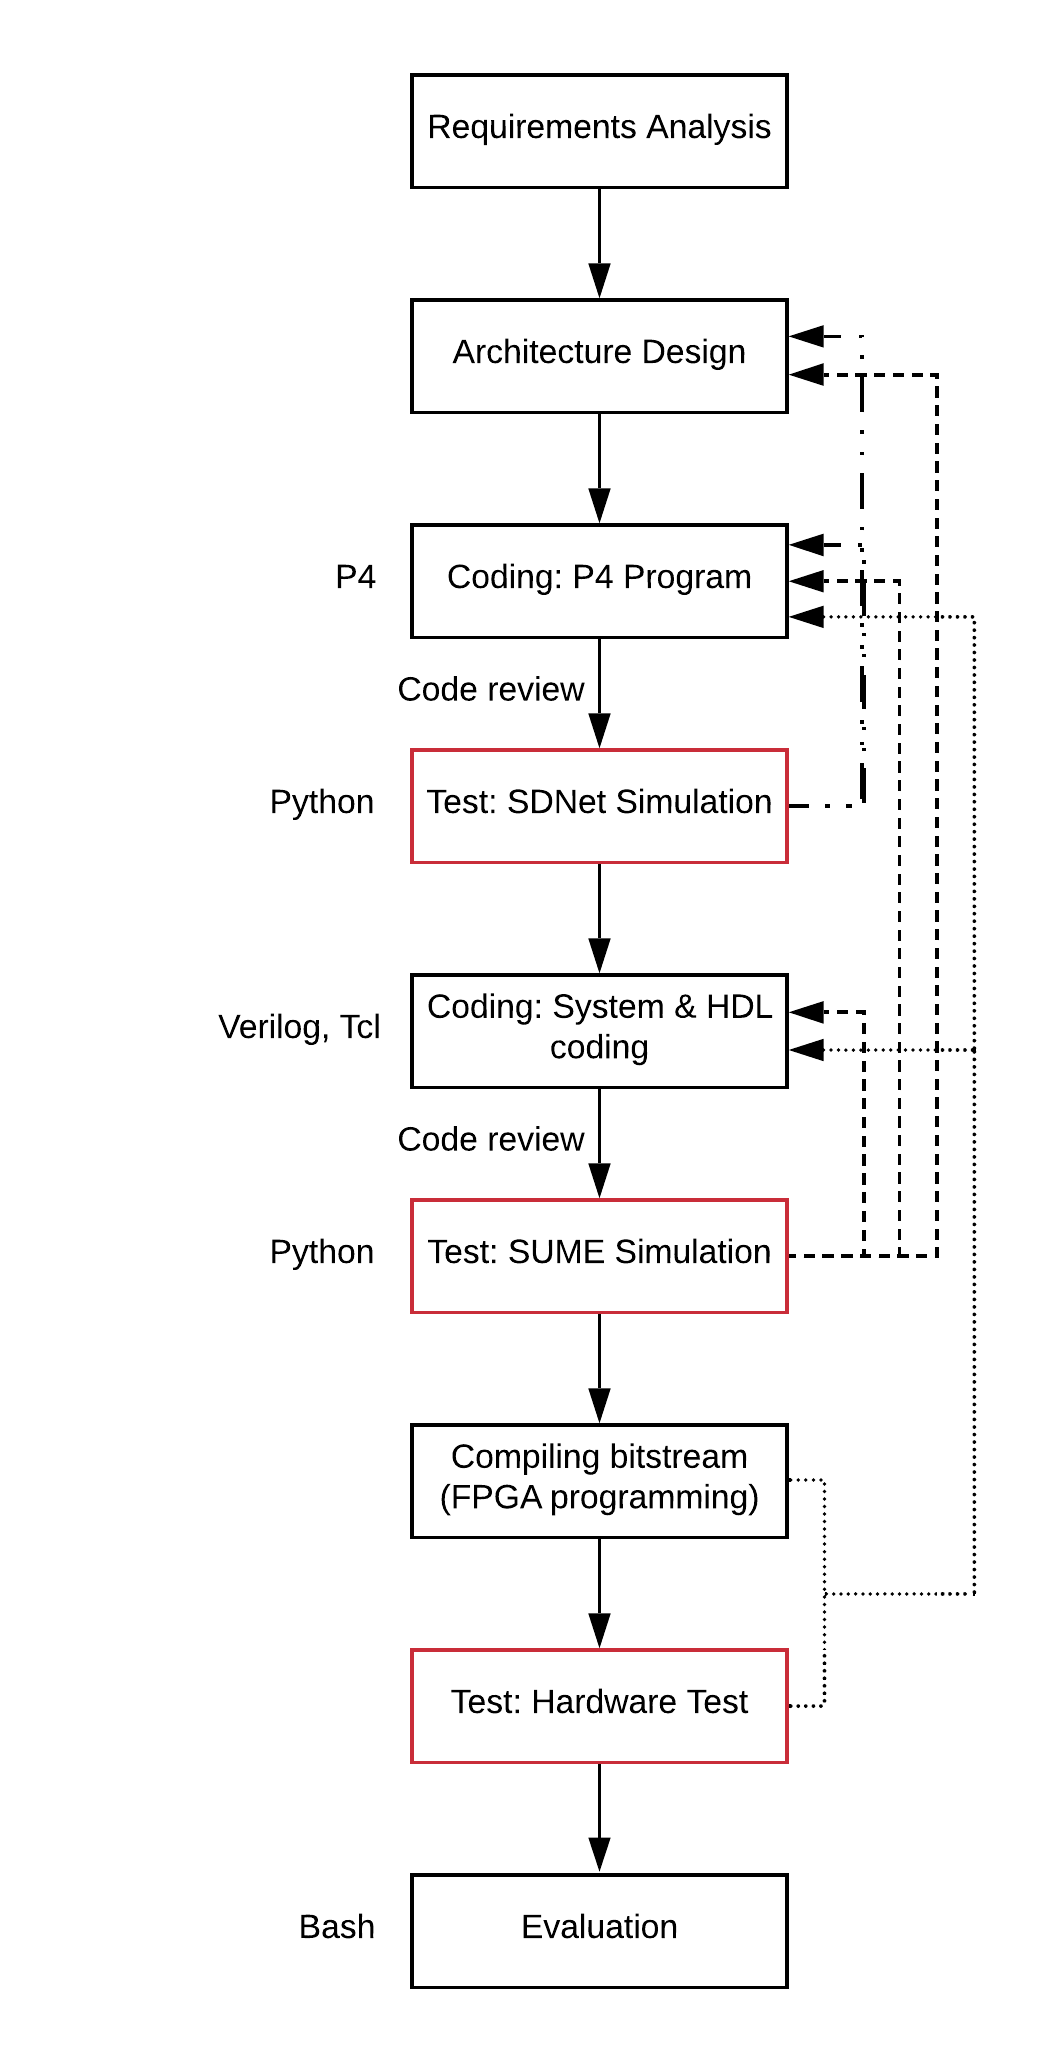
\includegraphics[width=0.75\textwidth]{workflow.png}
		\caption{Block diagram showing the workflow of the implementation stage. Dotted arrows represent a revision of previous steps, possibly with adjustments/refinements, in an iterative approach. Where appropriate, the programming language involved is stated. Passing all the steps in red box indicates the design meeting the requirements.}
		\label{fig:workflow}
	\end{figure}
	
	\subsection{Risk Analysis}
	The P4$\rightarrow$NetFPGA workflow is a complex platform that required the knowledge of a multitude of languages, with limited documentation \cite{fpga} and community support \cite{support}. A potential risk for the project was the difficulty of being sufficiently proficient with the platform to modify its core components and hence the inability to implement the design. Complete failure to do so was unlikely, but it could have consumed a significant amount of development time. As suggested by the spiral development model \cite{spiral}, this high-risk part was scheduled early and some “catch-up” time was allocated in the project timetable in case it caused significant delays.
	
	\subsection{Backup Plan}	
	Throughout the project development, I made sure to follow good backup procedure by keeping local weekly backups of my project using Time Machine for macOS. This provides recent history through incremental backups. I ensured additional remote storage by backing up with Microsoft OneDrive and Git, which also provided version control.
\chapter{Implementation}

\section{The SimpleSumeSwitch Architecture}
This project will work mainly with a NetFPGA SUME board \cite{zilberman2014netfpga}, using P4 programming language. I will be using the P4-NetFPGA workflow, which provides infrastructure to compile P4 programs to NetFPGA \cite{fpga}. Apart from that, everything else will be built from scratch.

I have no prior experience with either NetFPGA or P4, but this will be mitigated through self-learning in which I will make use of the online tutorials, Google's resources and the P4 community documentation, as well as the experience of my supervisors. 

\section{The Cache Queue}
The relevant Tripos courses that can serve as a starting point for this project are primarily: \emph{Computer Networking}, \emph{Principles of Communications} and \emph{ECAD and Architecture Practical Classes}. Since the courses are introductory, I will also consult Part III's \emph{High Performance Networking} course. I also plan to bridge any knowledge gap through extensive personal reading as well as help from my project supervisor.
%\section{}
\chapter{Evaluation}
\textit{This chapter assesses the functionality of my implementation in simulation and in hardware with regard to the initial requirements. I then evaluate the performance of my design. Finally, I compare its performance to existing TCP fast retransmit mechanism.}

The objective of this chapter is to review Unbuckle’s success at meeting the original project success criteria and at delivering benefits over state-of-the-art key-value stores. Hence, I begin by discussing the original project success criteria and how Unbuckle meets (and exceeds) them. Then, I briefly discuss the testing strategies applied. An extensive quantitative evaluation to assess the performance impact of various optimisations is carried out. Finally, I compare the user-space and kernel versions of Unbuckle, and show that it outperforms contemporary optimised commercial key- value stores. Comparisons against research systems are also made, where I find Unbuckle is competitive.

\section{Simulation Environment}
It is generally easier to debug program behaviour in simulation than in hardware, and the purpose of the simulation environment is exactly that. For this purpose, the P4$\rightarrow$NetFPGA workflow provides a simulation environment with automated test benches. To run a simulation, we will provide the corresponding test bench with the testing scripts. We will modify the following files:

\begin{itemize}
	\item \texttt{commands.txt} contains the set of commands to add entries to the match-action tables that we have defined in our P4 program (see Table \ref{}). These entries will be automatically added to the P4 tables at the start of each simulation. 
	\item \texttt{gen\_testdata.py} generates test packets (\& metadata), along with the corresponding expected output packets and metadata.
	\item \texttt{run.py} reads the test packets generated by the \texttt{gen\_testdata.py} script and applies the packets to the SUME interfaces.
\end{itemize}

The \texttt{gen\_testdata.py} template provided by the P4$\rightarrow$NetFPGA workflow has two functions--- \verb|applyPkt()| and \verb|expPkt()|---which allow us to specify input packets and expected output packets respectively. I wrote the \verb|digest_data.py| module and use Python \texttt{scapy} module to generate the metadata and test packets. The following code sequence shows an example of how to create and send a test packet, and specify the expected packet. We create the test packet using \texttt{scapy}'s \texttt{Ether}, \texttt{IP} and \texttt{TCP} classes, stacking the layer using the \texttt{/} operator and pad it to 64 bytes using \texttt{pad\_pkt()} method. Then, \verb|applyPkt()| will ``send'' the packet to the SimpleSumeSwitch module. Now, we need to specify how we would expect the output packet. We create two variables, \verb|flow_id| and \verb|actions|, to represent the value of the flow number and the \texttt{tuser} bus of the output packet. Finally, we use \verb|expPkt()| to put the packet into a list of ``expect'' packets.

{\renewcommand{\baselinestretch}{0.8}\small
	\begin{verbatim}
    from scapy.all import *
    from digest_data import *
	
    MAC_src = "08:11:11:11:11:08"  # nf0
    MAC_dst = "08:22:22:22:22:08"  # nf1
    sport = 55
    dport = 75
    IP_src = "10.0.0.1"
    IP_dst = "10.0.0.2"
	
    pkt = (
      Ether(src=MAC_src, dst=MAC_dst)
      / IP(src=IP_src, dst=IP_dst)
      / TCP(sport=sport, dport=dport, flags="S", seq=1)
    )                              # create the packet using scapy Ether, IP and TCP classes.
    pkt = pad_pkt(pkt, 64)         # pad the packet to 64 bytes
    applyPkt(pkt, "nf0", 0)        # send from port 0

    # compute the flow number
    flow_id = compute_flow_number(IP1_src, IP1_dst, 6, sport, dport)
    
    # write to port 1 of cache_queue
    actions = compute_tuser(0, 0, 0, tuser_map["nf1"])             
    
    # expect from port 1 of output_queue
    expPkt(pkt, "nf1", drop=False, flow_id=flow_id, tuser=actions)
	\end{verbatim}
}

Once the packets and metadata have been produced, we run two stages of simulation: SDNet simulation and SUME simulation.

\subsection{SDNet Simulation}
The SDNet simulation will compile the P4 code and simulate its behaviour. It is done by running the test bench produced by the SDNet compiler. This will first compile the code. After successful compilation, it then ``send'' the user defined input packets and metadata to the SimpleSumeSwitch HDL module and compare the outputs with the expected outputs. 

To simulate the behaviour of our switch under different scenarios, I wrote five test cases which I will now discuss the goal and the description of the test case, and present the output. For the purpose of the simulation, our flow of interest will be from MAC address \texttt{08:11:11:11:11:08}, IP address \texttt{10.0.0.1} and port 55 to MAC address \texttt{08:22:22:22:22:08}, IP address \texttt{10.0.0.2} and port 75.

NOTE: Show snapshots of the wave windows with arrows pointing to different important indications. I have not finished this. I will take snapshots of relevant part and put here. Would you prefer writing the test case in prose or in bullet points 

The first test case simulates the basic packet forwarding of the P4 program. We send one packet from port 0 to port 1 and expect to receive one packet coming out of port 1 of the SimpleSumeSwitch module. This packet should have:
\begin{itemize}
	\item The \verb|digest_data.flow_id| field computed to the binary representation of the flow number of the packet. Every packet that comes through the SimpleSumeSwitch module should have its flow number computed to decide whether it is the packet of the flow of interest.
	\item The \verb|digest_data.tuser| set to write the packet to the port 1 of the cache queue. Since this packet is of the flow of interest, we need to cache it to retransmit if necessary. 
\end{itemize} 

OR

Test \#1: Basic packet forwarding of the SimpleSumeSwitch-architecture-based P4 program
Goal: A packet coming through the SSS architecture will come out with the \texttt{digest\_data} modified.
Description:
\begin{itemize}
\item Send 1 packet from port 0 to port 1.
\item Expect 1 packet coming out of port 1 of the SSS with the \texttt{digest\_data.flow\_id} computed and matches the flow number of the original packet, and the \texttt{digest\_data.tuser} set to write the packet to the cache queue of port 1.
\end{itemize}

%\begin{figure}[!ht]
%	\centering
%	\includegraphics[width=\textwidth]{test1.png}
%	\caption{Test \#1: Basic packet forwarding of the SimpleSumeSwitch architecture-based P4 program.}
%	\label{test1}
%\end{figure}

The second test case.
%\begin{figure}[!ht]
%	\centering
%	\includegraphics[width=\textwidth]{test2.png}
%	\caption{Test \#2: Behaviour of the program when it receives a standard ACK packet.}
%	\label{test2}
%\end{figure}

The third test case.
%\begin{figure}[!ht]
%	\centering
%	\includegraphics[width=\textwidth]{test3.png}
%	\caption{Test \#3: Behaviour of the program when three DUP ACK packets are received.}
%	\label{test3}
%\end{figure}

The fourth test case.
%\begin{figure}[!ht]
%	\centering
%	\includegraphics[width=\textwidth]{test4.png}
%	\caption{Test \#4: Behaviour of the program when a fourth DUP ACK is received.}
%	\label{test4}
%\end{figure}

The fifth test case.
%\begin{figure}[!ht]
%	\centering
%	\includegraphics[width=\textwidth]{test5.png}
%	\caption{Test \#5: Behaviour of the program when there are multiple flows.}
%	\label{test5}
%\end{figure}

\subsection{SUME simulation}
Once the code passes the SDNet simulation (i.e. the actual outputs are the same as the expected outputs), the SUME simulation will install the SimpleSumeSwitch HDL module as a NetFPGA IP core and simulate the behaviour of the entire NetFPGA reference switch design. This simulation can also be done by running another test bench produced by the P4-SDNet toolchain. It uses the same stimuli and comparisons to verify that the SimpleSumeSwitch module was successfully integrated into our modified reference switch pipeline. 

The same five test cases were used to simulate the switch behaviour in our reference design, with the output shows success. The only noticeable difference is in test case \#4. 

\section{Hardware Test}
After all simulations indicate that the program is behaving correctly, the hardware test allows the design to be tested on the NetFPGA SUME board. 

I built the FPGA bitstream and started testing the design on hardware.

\section{Performance Evaluation}
\section{Comparison with TCP}


\chapter{Conclusion}
\section{Accomplishments}
Overall, the project achieved its aim of implementing and evaluating a programmable switch that is capable of assisting the fast retransmit process of TCP. The switch functionalities were evaluated in two different environments: a simulation environment and a hardware test. 

With the benefit of hindsight, I would have implemented the architecture prior to starting the project and used it as the starting point. This would have enabled me to focus more on evaluating and give more time to explore useful extensions.

\section{Future Work}

Many promising avenues for further improvement were not explored due to time constraints:

\begin{itemize}
	\item \textbf{Supporting multiple packet sizes}. The current design only supports a single packet size, defined at configuration time. It would definitely be more useful if the design could support multiple packet sizes dynamically, without first specifying them.
	
	\item \textbf{Supporting multiple flows}. It would also be useful to have one programmable switch to serve different applications between the same sender and receiver. The current design only supports one single flow since it only has one cache queue. Adding more cache queues would require a more complicated mechanism to signal a specific cache queue. 
	
	\item \textbf{Dynamic configuration}. The configurations of the flow and the packet size are currently pre-defined and embedded within the P4 code. A more flexible design could allow the user to adaptively installing and removing flows to monitor, as well as to configure the flow. 
	
\end{itemize}

\paragraph{Closing Remarks}\ 

This project has been a fascinating opportunity to explore the field of computer networking, especially high-performance networking, comprehend and appreciate the intricacy of TCP congestion control mechanism and the potential of data plane programmability. The project has achieved most of its goals and attempted to investigate and evaluate a modification to assist TCP fast retransmit algorithm, providing a starting point for future improvements. This project has also contributed to my personal development by improving my software engineering and technical writing skills.

% ******************************** Bibliography  *********************************

\pagestyle{plain}
\nocite{*}
\bibliographystyle{IEEEtranN}
\bibliography{References/references}

% ******************************** Appendix *********************************

\appendix

\chapter{Repository Overview}
\label{sec:repo}
The project repository comprises four main folders:\\
		\dirtree{%
			.1 P4-NetFPGA.
			.2 contrib-projects.
			.2 docs.
			.2 lib.
			.2 tools.
		}
\begin{itemize}[leftmargin=*, noitemsep]
	\item \texttt{contrib-projects}: contains the reference switch pipeline, the core logic of the switch in P4 and the testing scripts.
	\item \verb|docs|: contains design documentations and user-guides.
	\item \texttt{lib}: contains custom and reference IP Cores and software libraries.
	\item \verb|tools|: contains scripts for automations: running simulations, etc.
\end{itemize}

The \verb|contrib-projects|, \verb|lib| and \verb|tools| folders contain the P4 (*) and Verilog (**) implementation of the design:\\
\dirtree{%
	.1 contrib-projects.
		.2 sume\_sdnet\_switch/projects/tcp\_retransmit.
			.3 simple\_sume\_switch/hw.
				.4 hdl/nf\_datapath.v**.
				.4 tcl.
					.5 simple\_sume\_switch.tcl.
					.5 simple\_sume\_switch\_sim.tcl.
			.3 test/sim\_switch\_default.
				.4 run.py**.
		.2 src.
			.3 tcp\_retransmit.p4*.
			.3 commands.txt*.
		.2 testdata.
			.3 gen\_testdata.py*.
			.3 digest\_data.py*.
			.3 sss\_sdnet\_tuples.py*.
		.2 templates.
			.3 externs/<externs\_type>/hdl/<externs\_type>\_template.v**.
}
\vspace*{5mm}
\dirtree{%
	.1 lib.
		.2 hw.
			.3 contrib/cores.
				.4 sss\_cache\_queues\_v1\_0\_0**.
			.3 std/cores.
				.4 output\_arbiter\_v1\_0\_0**.
}
\vspace*{5mm}
\dirtree{%
	.1 tools.
		.2 scripts/NFTest/nf\_test.py**.
}

\chapter{Figures and Tables}
\label{sec:figures}
Appendix \ref{sec:figures} contains Figures and Tables that are not specific to the project, but were referred to in the dissertation.

\begin{figure}[h]
	\centering
	\begin{subfigure}[b]{\textwidth}
		\centering
		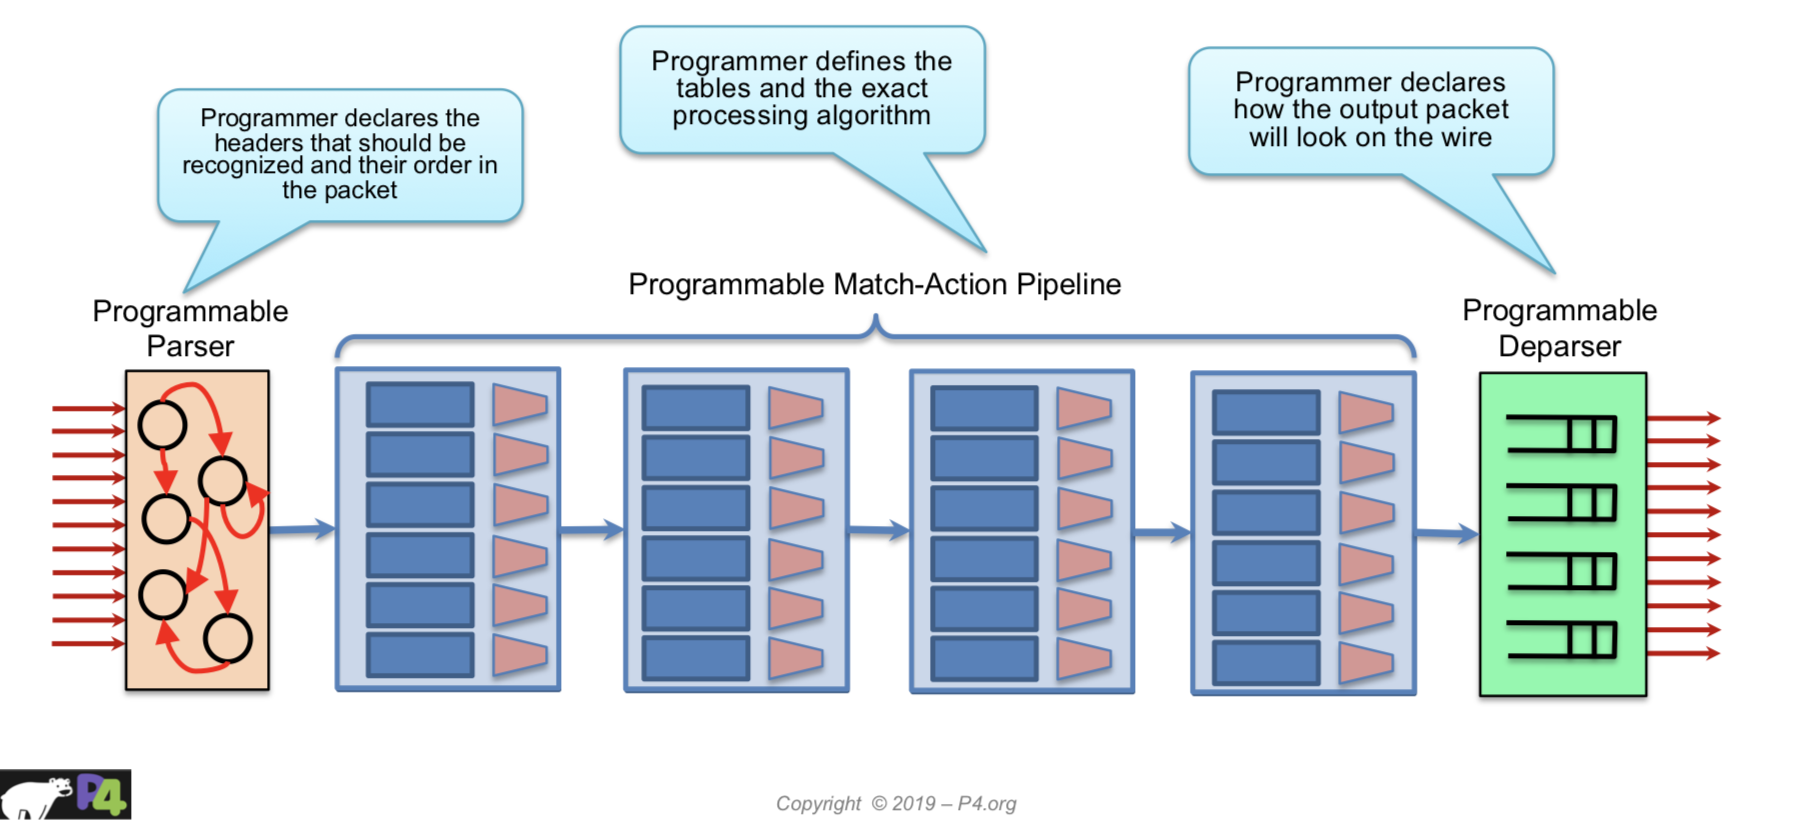
\includegraphics[width=\textwidth]{pisa.png}
		\caption{The single programmable pipeline forwarding architecture of PISA.}
		\label{fig:pisa}
	\end{subfigure}
	
	\vspace*{5mm}
	
	\begin{subfigure}[b]{\textwidth}
		\centering
		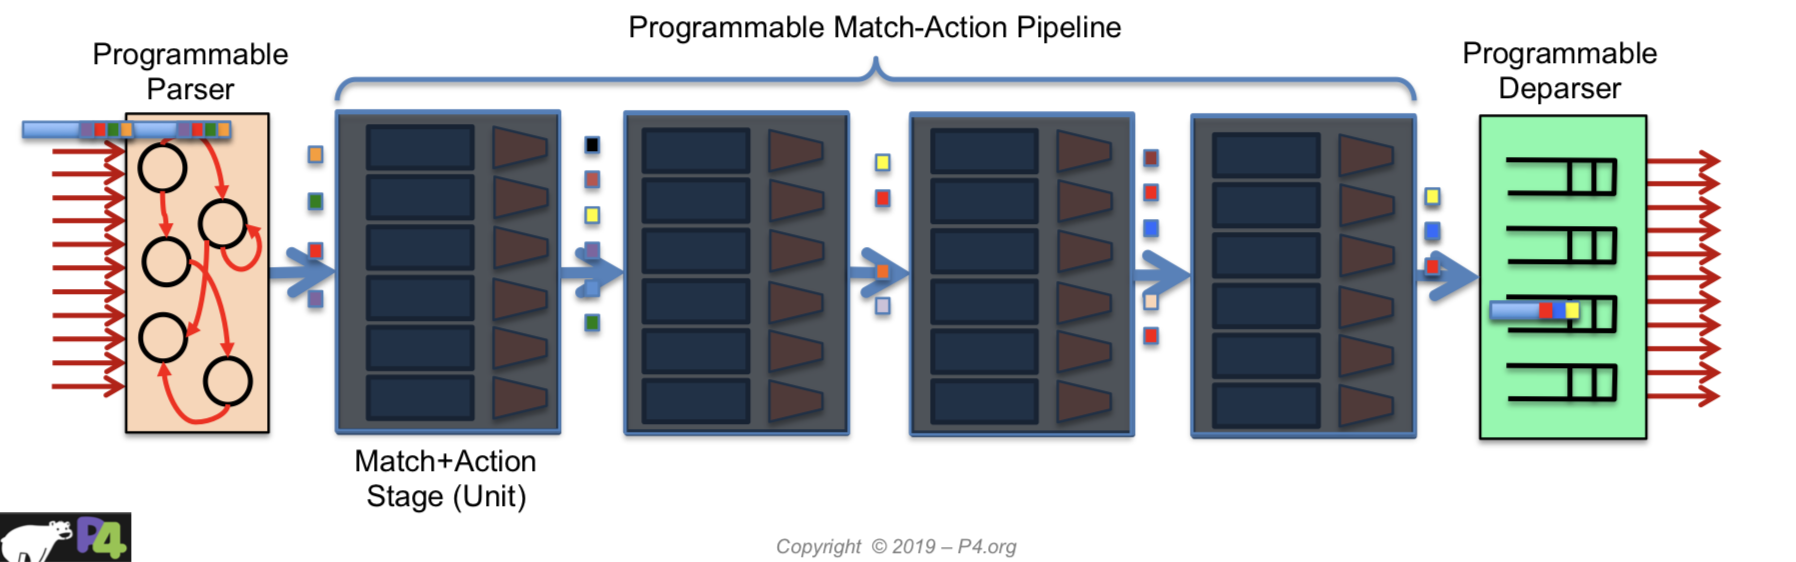
\includegraphics[width=\textwidth]{pisa1.png}
		\caption{The life cycle of a packet going through the PISA pipeline.}
		\label{fig:pisa1}
	\end{subfigure}
	\caption{PISA---Protocol-Independent Switch Architecture. Source: \href{https://p4.org}{P4.org -- Copyright \textcopyright\ 2019}.}
\end{figure}

\begin{table}[!ht]
	\begin{center}
		\caption{The P4$\rightarrow$NetFPGA extern functions library.}
		\label{tab:externs}
		\begin{tabular}{ | c | c | }
			\hline
			\multicolumn{2}{|c|}{\textbf{Stateful Atomic Extern Functions}} \\ \hline
			\textbf{Type} & \textbf{Description}  \\ \hline
			RW & Read or write state \\ \hline
			RAW & Read, add to, or overwrite state  \\ \hline
			PRAW & Either perform RAW or do not perform RAW based on predicate \\ \hline
			ifElseRAW & Two RAWs, one each for when a predicate is true or false \\ \hline
			Sub & IfElseRAW with stateful subtraction capability \\ \hline
			
			\multicolumn{2}{|c|}{\textbf{Stateless Extern Functions}} \\ \hline
			\textbf{Type} & \textbf{Description}  \\ \hline
			IP Checksum & Given an IP header, compute the IP checksum \\ \hline
			LRC & Longitudinal redundancy check, simple hash function \\ \hline
			timestamp & Generate timestamp (measured in clock cycles, granularity of 5ns) \\ \hline
		\end{tabular}
	\end{center}
\end{table}

\begin{figure}[!h]
	\centering
	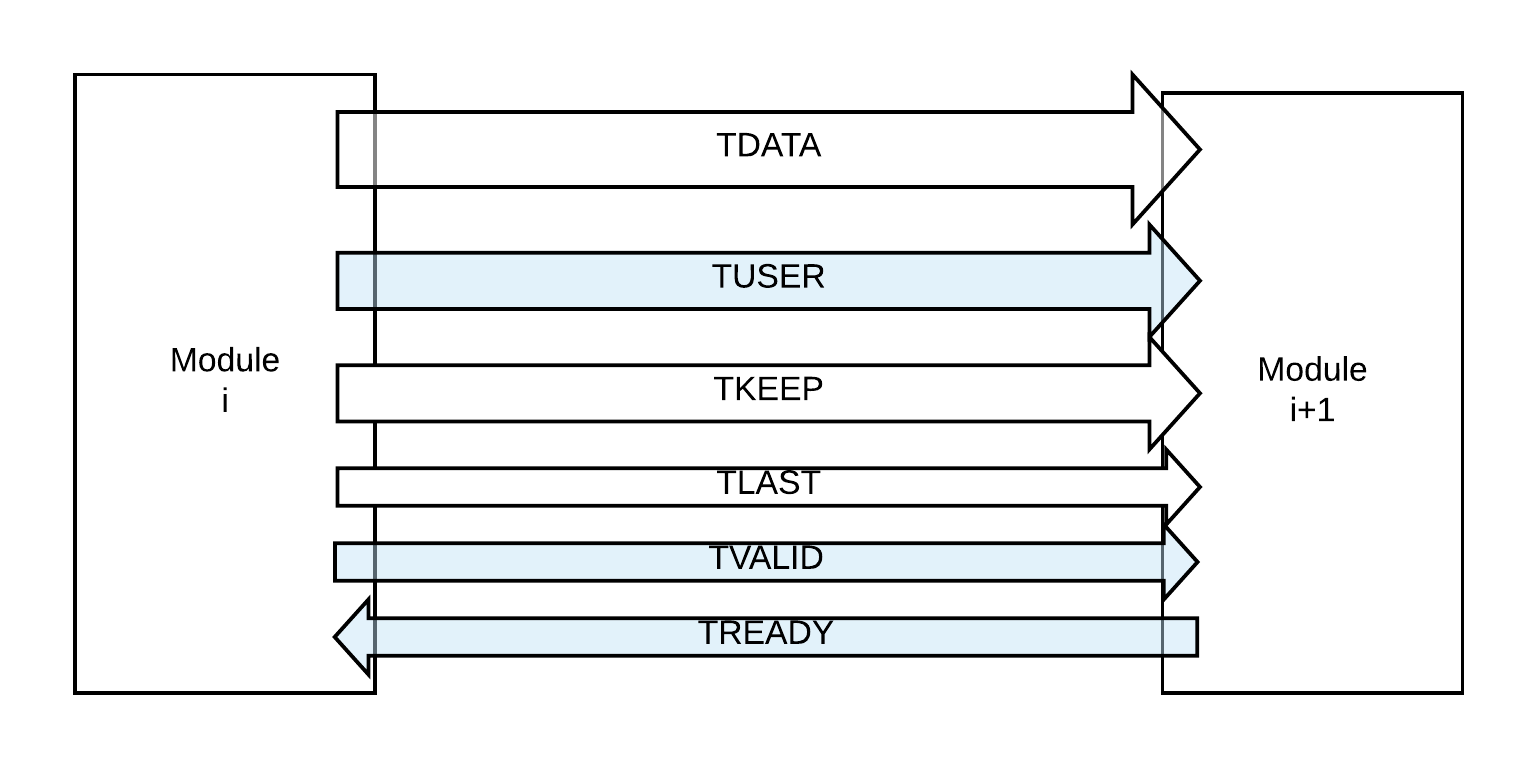
\includegraphics[width=0.85\textwidth]{axi.png}
	\caption{Inter-module communication is done via AXI-4 streams (Packets are moved as stream).}
	\label{fig:axi}
\end{figure}

\begin{table}[!h]
	\centering
	\caption{The AXI-4 streams and their descriptions.}
	\label{tab:axi}
	\begin{tabular}{ | l | l |}
		\hline
		\textbf{AXI-4 Stream} & \textbf{Description} \\ \hline
		TDATA & Data stream \\ \hline
		TKEEP & Marks NULL bytes (i.e. byte enable) \\ \hline
		TVALID & Validity indication \\ \hline
		TREADY & Flow control indication \\ \hline
		TLAST & End of packet/burst indication \\ \hline
		TUSER & Sideband metadata \\ \hline
	\end{tabular}
\end{table}

\chapter{Reproducibility}
\label{sec:reproduce}
Appendix \ref{sec:reproduce} gives the specification of the test machine and the required software and equiment to reproduce the results presented in the dissertation.
\section{Test Machine}
The following machine, software and equipment were used:
\begin{itemize}[leftmargin=*, noitemsep]
	\item A PC with Ubuntu 14.04.5 LTS (GNU/Linux 4.4.0-83-generic x86\_64).
	\item Xilinx Vivado 2018.2 (License)
	\item Xilinx P4-SDNet (License)
	\item Xilinx 10G MAC (License)
	\item The NetFPGA SUME board.
\end{itemize}
\section{Scripts}
The steps to reproduce the SDNet simulation, SUME simulation and hardware-based test are as followed:
\begin{enumerate}[leftmargin=*, noitemsep]
	\item Go to the repository:\\
{\centering	\verb|cd P4-NetFPGA/|}
	\item Update the environment variables:\\
	 \verb|source tools/setting.sh|
	\item To run both the SDNet and SUME simulation:\\
	 \verb|cd $P4_DESIGN_DIR && make workflow|
	\item To run the SDNet simulation only:\\
	 \verb|cd $P4_DESIGN_DIR && make vivado_sim|
	\item To run the SUME simulation only:\\
	 \verb|cd $P4_DESIGN_DIR && make sume_sim|
	\item Once the SUME simulation finishes, to run the hardware test:\\
	 \verb|cd $SUME_FOLDER| \\
	 \verb|./tools/scripts/nf_test.py hw --major switch --minor default|
	\item Once the hardware test finishes, to compile the bitstream for FPGA:\\
	 \verb|cd $NF_DESIGN_DIR && make|
\end{enumerate}


\chapter{Project Proposal}
\label{sec:proposal}
\setlength{\parskip}{0.75\baselineskip}

\maketitlep

% ******************************** Main Proposal *********************************

\chapter{Introduction}
\textit{In this chapter, I provide the motivation for this project and setup the problem I am solving. I also explain some key algorithms involved. Finally, I cover some related work.}

\section{Motivation}
	
 Transmission Control Protocol (TCP) is the protocol of choice in many data centers. However, it is very sensitive to losses (by design, as a mean for congestion control), which can degrade the performance within the data centers significantly \cite{zilberman2017has}. Various congestion control, avoidance and recovery mechanisms are thus of high importance in this field to minimise such loss rate. Still, not all TCP losses are born equal. For example, losses happening at the destination host's network interface card (NIC) are not an indication of congestion within the network. It is assumed that fast retransmission of such lost packets, from within the network, can increase the utilization of the network.
 
 In-network computing is an emerging research area in systems and networking, where applications traditionally running on the host are offloaded to the network hardware (e.g. switch, NIC). Examples of applications offloaded in the past include network functions (DNS server \cite{dns}), distributed systems functions such as consensus (P4xos \cite{p4xos}), various caching (netCache \cite{netCache}, netChain \cite{netChain}) and even a game (Tic-Tac-Toe). Key-Value Store (KVS) is also among the popular type of in-network applications. 
 
 Therefore, it is particularly interesting, and indeed challenging, to see how network-accelerated KVS concepts can be applied to TCP fast retransmit mechanism in order to improve cross-datacentre performance.
 
\section{Project Aims}
Fast retransmit is an enhancement to TCP that reduces the time a sender waits before retransmitting a lost segment. A TCP sender normally uses a simple timer to recognize lost segments. If an acknowledgement is not received for a particular segment within a specified time (a function of the estimated round-trip delay time), the sender will assume the segment was lost in the network, and will retransmit the segment.

Duplicate acknowledgement (DUP ACK) is the basis for the fast retransmit mechanism. After receiving a packet (e.g. with sequence number 1), the receiver sends an acknowledgement by adding 1 to the sequence number (i.e. acknowledgement number 2). This indicates to the sender that the receiver received the packet number 1 and it expects packet number 2. Suppose that three subsequent packets are lost. The next packets the receiver sees are packet numbers 5 and 6. After receiving packet number 5, the receiver sends an acknowledgement, but still only for sequence number 2. When the receiver receives packet number 6, it sends yet another acknowledgement value of 2. Duplicate acknowledgement occurs when the sender receives more than one acknowledgement with the same sequence number (2 in our example).

When a sender receives several DUP ACKs, it can be reasonably confident that the segment with the sequence number specified in the DUP ACK was dropped. A sender with fast retransmit will then retransmit this packet immediately without waiting for its timeout.

\begin{figure}[h]
	\centering
	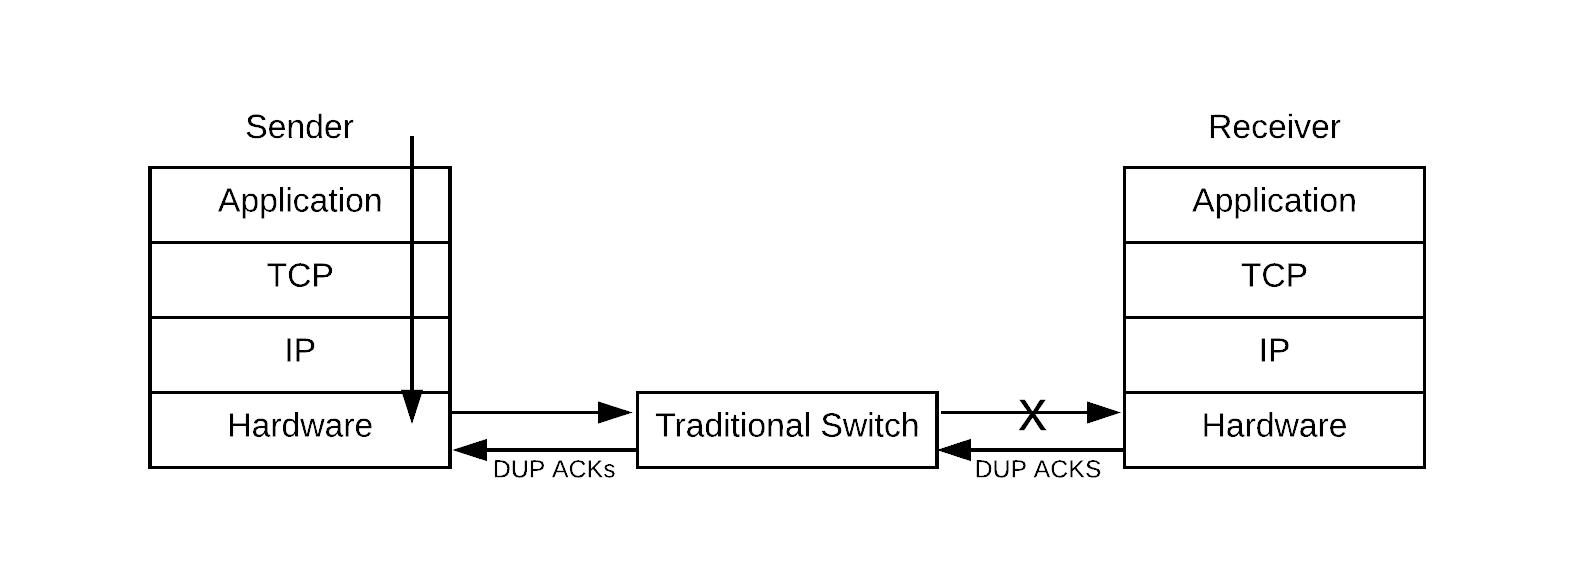
\includegraphics[width=\textwidth]{tradition-tcp.png}
	\caption{The standard convention of TCP handling.}
	\label{tradition-tcp}
\end{figure}

Currently, the DUP ACKs will traverse all the way back to the sender (\textbf{Figure \ref{tradition-tcp}}). The sender receives the DUP ACKs, then retransmits the packet with the next higher sequence number. 

\begin{figure}[h]
	\centering
	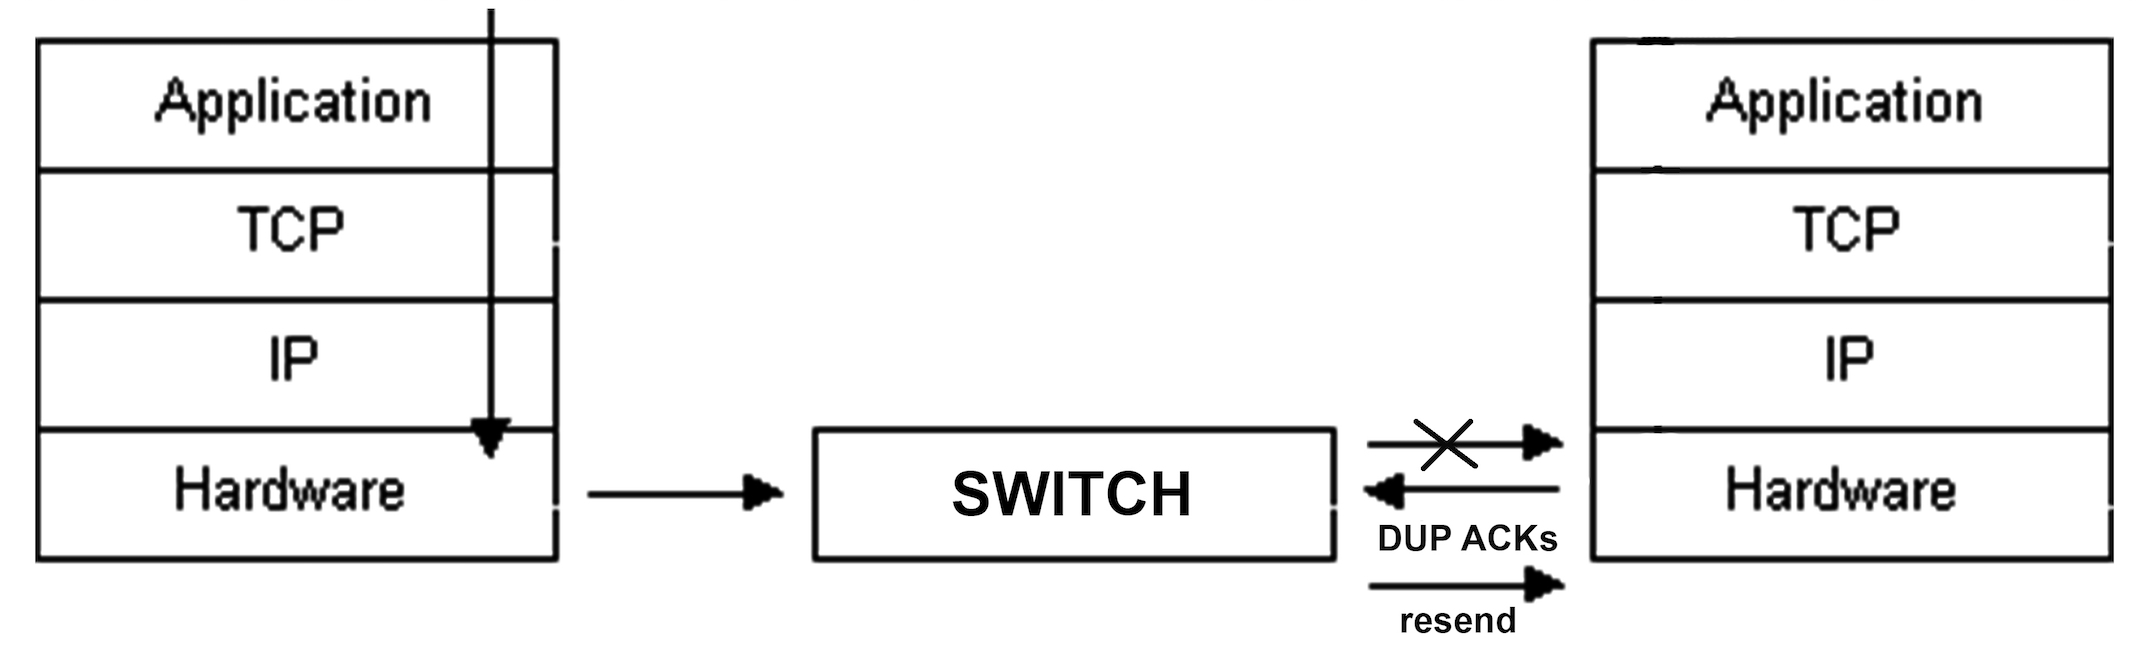
\includegraphics[width=\textwidth]{project-tcp.png}
	\caption{The proposed TCP handling.}
	\label{project-tcp}
\end{figure}

This project aims to design and implement a programmable switch that assists the TCP fast retransmit algorithm. The programmable switch will be able to retransmit the packets from within the network, instead of waiting for the DUP ACKs to get back to the host (\textbf{Figure \ref{project-tcp}}), thereby aims to reduce the response time to DUP ACKs and reduce unnecessary changes to the congestion window. The implementation will be based on the KVS concept, where the keys are the flow ID and the packet sequence number, and the value is the payload.

\section{Related Work}
	\subsection{TCP Congestion Control}
	One of the main aspects of TCP is congestion control, where a number of mechanisms are used to achieve high performance and avoid sending more data than the network is capable of forwarding, that is, to avoid causing network congestion. In particular, TCP uses a \textit{congestion avoidance} algorithm that includes various aspects of an additive increase/multiplicative decrease (AIMD) scheme, with other schemes such as \textit{slow start}, \textit{fast retransmit} and \textit{fast recovery} to achieve congestion avoidance. 
	
	The four intertwined algorithms are defined in more detail in RFC 5681\cite{rfc5681}. In this project, we are mostly interested in the \textit{fast retransmit} algorithm, which has been explained in the previous section.
	
	\subsection{Programmable Data Planes}
	The use of P4, netFPGA, etc.


\section*{\fontsize{18pt}{0.5}\selectfont Starting Point}

\subsection*{Platform \& Language}
This project will work mainly with a NetFPGA SUME board \cite{netfpgasume}, using P4 programming language. I will be using the P4-NetFPGA workflow, which provides infrastructure to compile P4 programs to NetFPGA \cite{fpga}. Apart from that, everything else will be built from scratch.

I have no prior experience with either NetFPGA or P4, but this will be mitigated through self-learning in which I will make use of the online tutorials, Google's resources and the P4 community documentation, as well as the experience of my supervisors. 

\subsection*{Computer Science Tripos}
The relevant Tripos courses that can serve as a starting point for this project are primarily: \emph{Computer Networking}, \emph{Principles of Communications} and \emph{ECAD and Architecture Practical Classes}. Since the courses are introductory, I will also consult Part III's \emph{High Performance Networking} course. I also plan to bridge any knowledge gap through extensive personal reading as well as help from my project supervisor.
\section*{\fontsize{18pt}{1}\selectfont Resources Required}

For this project I will be using my own computer, a 2017 MacBook Pro with a 2.3 GHz Intel Core i5 processor and 16 GB of RAM, that runs macOS Mojave. I accept full responsiblity for this machine, and I have made contingency plans to deal with hardware and/or software failures. Should that machine suddenly fail, I have another 16Gb of RAM computer with a 2.6 GHz Intel Core i7 processor that runs Ubuntu 18.04 LTS. If all else fails, I can continue to work on an MCS machine. Backups will be done weekly to Microsoft OneDrive and my external hardrive, and all my codes will be uploaded to GitHub for version control. 

For the hardware prototype, I will require a NetFPGA SUME board. I will need access to a machine that has the SUME installed, and a 10G NIC. These will be supplied by my supervisor. I will be using my own machine for development, with remote access to a server with the SUME board inside.

I will also require access to the lab network in order to \emph{ssh} to the server with the SUME board. Development on my machine will require VPN access, for using floating licenses of the development tools. Lastly, I will require a second server for testing some of the extensions of the project.
\section*{\fontsize{18pt}{1}\selectfont Work to be Done}

The main core component of the project is to be able to apply the KVS concept, where the sequence number and flow Id of a packet are the key and the packet is the value, to implement TCP fast recovery. In order to do that, the following sub-tasks must be done:

\begin{enumerate}
	
	\item First, since the project is done on NetFPGA using P4 programming language, both of which I am not familar with, I first have to study them thoroughly and be proficient working with the platform.
	
	\item I would also need to study and gain a better understanding of KVS applications, TCP congestion control and recovery mechanisms, as well as their use cases (e.g. High Frequency Trading, in-datacenter latency sensitive applications, etc.).
	
	\item The next stage will be to design the architecture for the application. This is a non-trivial process. Generally, it will be to try to map the application to a match-action pipeline.
	
	\item The fourth stage involves implementing the architecture in code. The program, which will be written in P4, will have the basic functionalities such as:
	\begin{itemize}
		\item A basic L3 switch function and TCP decoding (send TCP, read the flow information from the table/register)
		
		\item Matching packets to a "\emph{key}" (its flow Id):
			\begin{itemize}
				\item If the key is of a new packet, store it (SET()).
				\item If the key is of a DUP ACK, read the packet and re-send (GET()).
				\item If the number of DUP ACKs is greater than $N$, do not resend. Instead, forward to host as the standard convention of handling TCP.
				\item Do not resend if the flow Id is not in a "selected" table. In other words, use the KVS only if the flow Id matches a predefined set of flow Ids, or a different predefined rule by the user.
			\end{itemize}		
	
	\end{itemize}
	
	\item \textbf{The simulation stage:} perform functionality test by simulating the program using bmv2 or Xilinx simulators to ensure correctness. 
	
	\item After it runs smoothly in the software, it will then be compiled to the hardware. Ensure that the basic functionalities mentioned above work in hardware.
	
	\item \textbf{The hardware stage:} demonstrate interoperability with a software-based client/application.
	
	Possibly, I will implement a drop $1:N$ packets at the server to force DUP ACKs, and I will also be using a synthetic benchmark such as \emph{multilate} \cite{multilate} -- a memcached benchmark -- or OSNT \cite{OSNT} as the applications on top of the network. The criterion to evaluate the performance is the flow completion time. There is no intention to use network simulators such as ns2, omnet++, etc. This is outside the scope of this project.
	
	The aim for this stage is to get a working prototype in hardware that supports a single flow and single packet size, and evaluate on its performance.
	
	\item Once the prototype is up and working, I need to implement further extensions to allows the prototype to support a variety of parameters/conditions (which will be discussed in \textbf{Possible Extensions} section).
		
\end{enumerate}

\section*{\fontsize{18pt}{1}\selectfont Success Criteria}

This project will be deemed a success if I managed to study and design an architecture for the application, as well as succeeded to implement that design. More concretely:

\begin{enumerate}
	\item I have an implementation of the application written in P4.
	
	\item The implementation works in simulation (using bmv2/Xilinx simulators).
	
	\item I have a working prototype. In other words, my design runs on the hardware.
	
	\item I am able to demonstrate interoperability with a software-based client/application.
	
	\item I can provide a performance evaluation of the design.
\end{enumerate}
\section*{\fontsize{18pt}{1}\selectfont Possible Extensions}

If the core parts of the project are successful and completed within a reasonable time, I shall then try to investigate and implement further extensions. Some possible options are:

\begin{enumerate}
	\item Supporting more than a single flow, and supporting the configuration of flows to monitor (\& retransmit)
	
	\item Supporting different packet sizes (depends on workflow limitations).
	
	\item Sending a notification to the source if multiple retransmits fail.
	
	\item Adaptively installing and deleting from the list of flows to monitor.
	
	\item A performance evaluation comparison to existing TCP recovery mechanisms.
\end{enumerate}
\section*{\fontsize{18pt}{1}\selectfont Timetable}

The schedule is broken into 15 2-week periods, with the first period starting on 19/10/2018.

\begin{enumerate}
	%1
	\item \textbf{Michaelmas weeks 2--4 [19/10--5/11]:} Preparatory reading on the P4 programming language and setting up the NetFPGA platform. Going through the tutorials and experimenting with some examples. Study TCP congestion control and recovery mechanisms beyond the material taught in \emph{Computer Networking} and \emph{Principles of Communications} courses.
	
	%2
	\item \textbf{Michaelmas weeks 5--6 [6/11--19/11]:} Design the architecture: mapping the application to a match-action pipeline.
	\\
	\textbf{\underline{Milestone:} Understand the application architecture. Be able to map the application to a match-action pipeline.}
	
	%3
	\item \textbf{Michaelmas weeks 7--8 [20/11--28/11]:} Start implementing of the design by writing the basic code. 
	
	%4
	\item \textbf{Michaelmas vacation weeks 1--2 [30/11--12/12]:} Simulate the application using bmv2/Xilinx simulators. 
	\\
	\textbf{\underline{Milestone:} Basic design written in P4 working in simulation, with minimal bugs left.} .
	
	%5
	\item \textbf{Michaelmas vacation weeks 3--4 [13/12--26/12]:} Start to implement the working code into hardware. Write a hardware-test program (Python-based). 
	
	%6
	\item \textbf{Michaelmas vacation weeks 5--7 [27/12--16/1]:} Demonstrate interoperability with a software-based client/application. Start writing the progress report.
	\\
	\textbf{\underline{Milestone:} Have the application working in hardware, a completed progress report and a presentation for demonstration purposes.}
	
	%7
	\item \textbf{Lent weeks 1--2 [17/1--30/1]:} Work on the design's performance testing and evaluation.
	
	%8
	\item \textbf{Lent weeks 3--4 [31/1--13/2]:} Continue working on testing and evaluation of the design.
	\\
	\textbf{\underline{Milestone:} The project is finished and meets the success criteria.}
	
	%9
	\item \textbf{Lent weeks 5--6 [14/2--27/2]:} Start working on extensions, based on project's progress.
	\\
	\textbf{\underline{Milestone:} The prototype continues to work well with the extensions implemented.}
	
	%10
	\item \textbf{Lent weeks 7--8 [28/2--13/3]:} Possible overflow from the previous weeks. Clean up codes and repository. Start writing dissertation main chapters.
	\\
	\textbf{\underline{Milestone:} Completed working prototype with core components and extensions in place. First draft of dissertation}
	
	%11
	%12	
	%13
	\item \textbf{Easter vacation:} Continue writing dissertation. Review cycles and corrections to dissertation towards the end of the vacation.
	
	%14
	\item \textbf{Easter weeks 1--2 [25/4--8/5]:}  Completed dissertation. Proof reading and then an early submission so as to concentrate on examination revision.
	
	%15
	\item \textbf{Easter weeks 3 [9/5--17/5]:} Buffer week.
\end{enumerate}


% ********************************************************************************

\end{document}